% =========================================================================
% CAPITOLO 3: CLASSIFICAZIONE (SPOTIFY)
% =========================================================================
\section{Spotify tracks analysis: Classificazione}

La classificazione supervisionata è stata condotta con l'obiettivo di sviluppare modelli predittivi in grado di determinare il genere musicale di ciascun brano a partire dalle sue caratteristiche audio. Il processo ha compreso una rigorosa fase di preprocessing e bilanciamento dei dati, la definizione di scenari sperimentali, l'addestramento e l'ottimizzazione degli iperparametri di molteplici algoritmi di apprendimento e, infine, l'integrazione di tecniche avanzate di \textit{Ensemble Learning}.

\subsection{Preprocessing del Dataset}

Per consentire una corretta valutazione empirica, il dataset ripulito di 35.877 brani è stato inizialmente suddiviso in Training Set (80\%, pari a 28.701 campioni) e Test Set (20\%, pari a 7.176 campioni), impiegando una procedura di campionamento stratificato per preservare le proporzioni originali delle classi.

Al fine di evitare qualunque forma di \textit{data leakage}, la standardizzazione delle feature è stata eseguita tramite \texttt{StandardScaler}, calcolando media e deviazione standard unicamente sui dati di addestramento:
\begin{equation}
z = \frac{x - \mu_{\text{train}}}{\sigma_{\text{train}}}
\label{eq:standardizzazione}
\end{equation}
I parametri $\mu_{\text{train}}$ e $\sigma_{\text{train}}$ ottenuti sono stati successivamente utilizzati per trasformare il test set senza ricalcolo.

\subsubsection{Oversampling con SMOTE e Undersampling}

Come evidenziato nel capitolo precedente, la distribuzione dei generi nel dataset originale risulta fortemente disomogenea. Per risolvere questo problema, è stata adottata una strategia ibrida di ricampionamento applicata \textbf{esclusivamente al dataset di training}:
\begin{itemize}
    \item \textbf{Oversampling con SMOTE (Synthetic Minority Over-sampling Technique):} Per le classi minoritarie (in particolare \textit{Pop}, \textit{Rap}, \textit{Emo}, \textit{RnB} e \textit{Trap Metal}), è stata impiegata la tecnica SMOTE. A differenza della semplice duplicazione casuale dei record (che favorisce l'overfitting), SMOTE seleziona i $k$-nearest neighbors di ciascun campione della classe minoritaria e genera nuove osservazioni sintetiche interpolando linearmente nello spazio continuo delle feature.
    \item \textbf{Undersampling Controllato:} Per le classi fortemente maggioritarie (come \textit{Underground Rap} e \textit{Dark Trap}), è stato eseguito un undersampling casuale per ridurne l'eccesso numerico ed evitare che dominassero la discesa del gradiente durante l'apprendimento.
\end{itemize}

\subsubsection{Dataset Finale}

Dopo l'applicazione congiunta di SMOTE e dell'undersampling, il training set bilanciato presenta esattamente \textbf{2.000 campioni per ciascuna delle 15 classi}, per un totale complessivo di \textbf{30.000 campioni bilanciati}. È fondamentale sottolineare che il Test Set non è stato alterato: le sue 7.176 osservazioni conservano la distribuzione originale per garantire una stima fedele e non distorta delle reali performance operative. La Figura \ref{fig:distribuzione_sampling} illustra il confronto tra le distribuzioni prima e dopo l'intervento di sampling.

\begin{figure}[H]
    \centering
    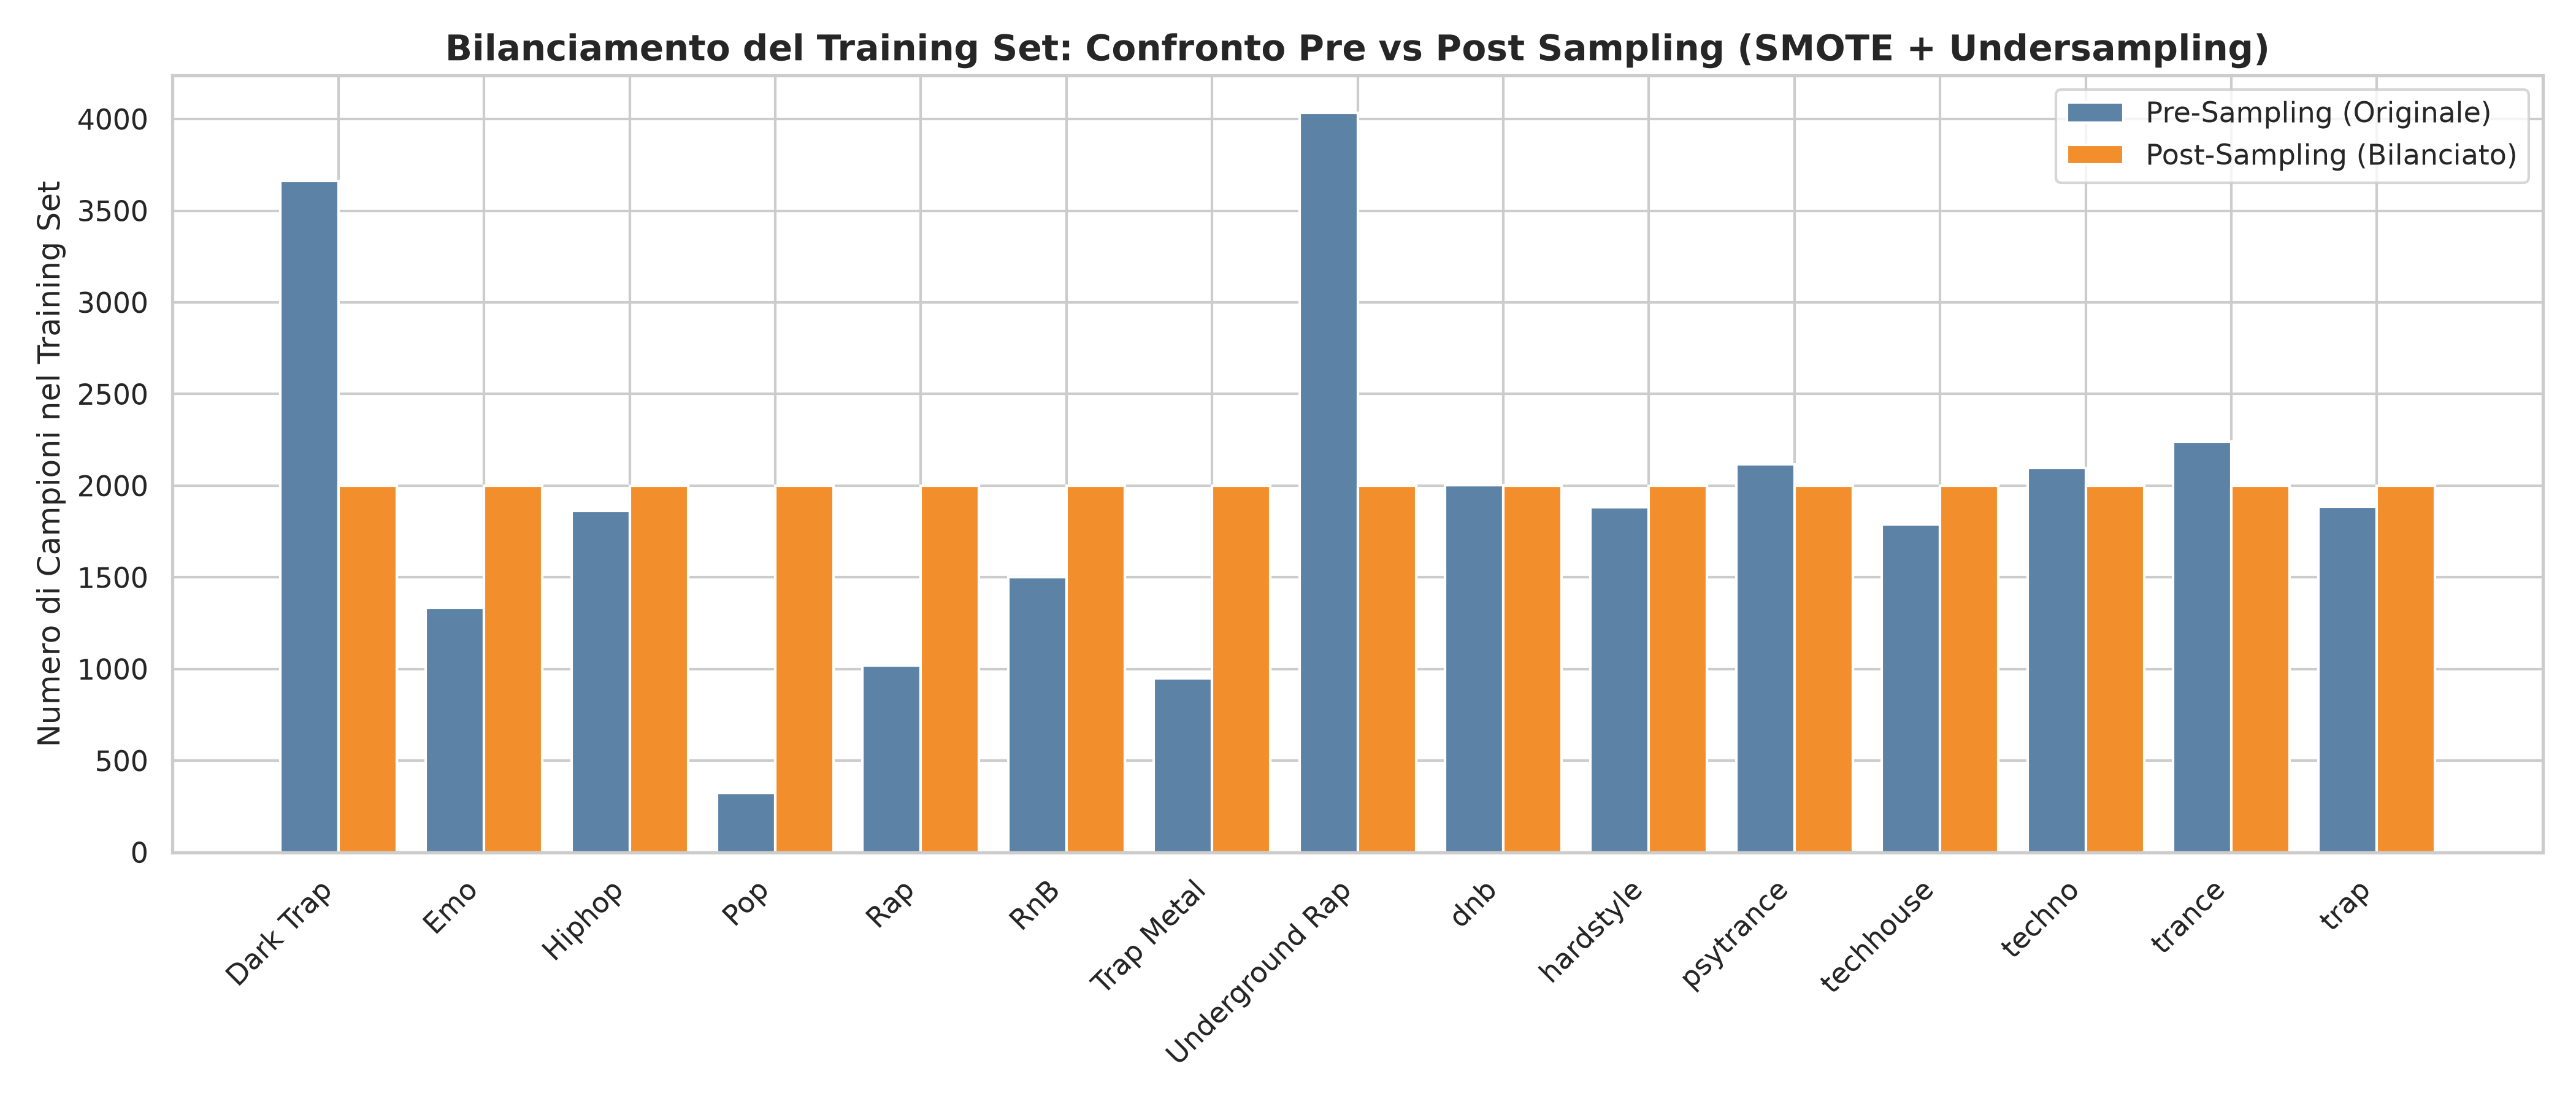
\includegraphics[width=0.88\textwidth]{capitolo3/img/fig05_distribuzione_sampling.png}
    \caption{Bilanciamento del Training Set: confronto della distribuzione delle classi pre vs post SMOTE e Undersampling.}
    \label{fig:distribuzione_sampling}
\end{figure}

Per verificare che la generazione di campioni sintetici non abbia introdotto correlazioni spurie alterando la struttura latente del segnale audio, è stata ricalcolata la matrice di correlazione di Pearson sui 30.000 campioni del training set post-sampling, mostrata in Figura \ref{fig:matrice_corr_post_sampling}.

\begin{figure}[H]
    \centering
    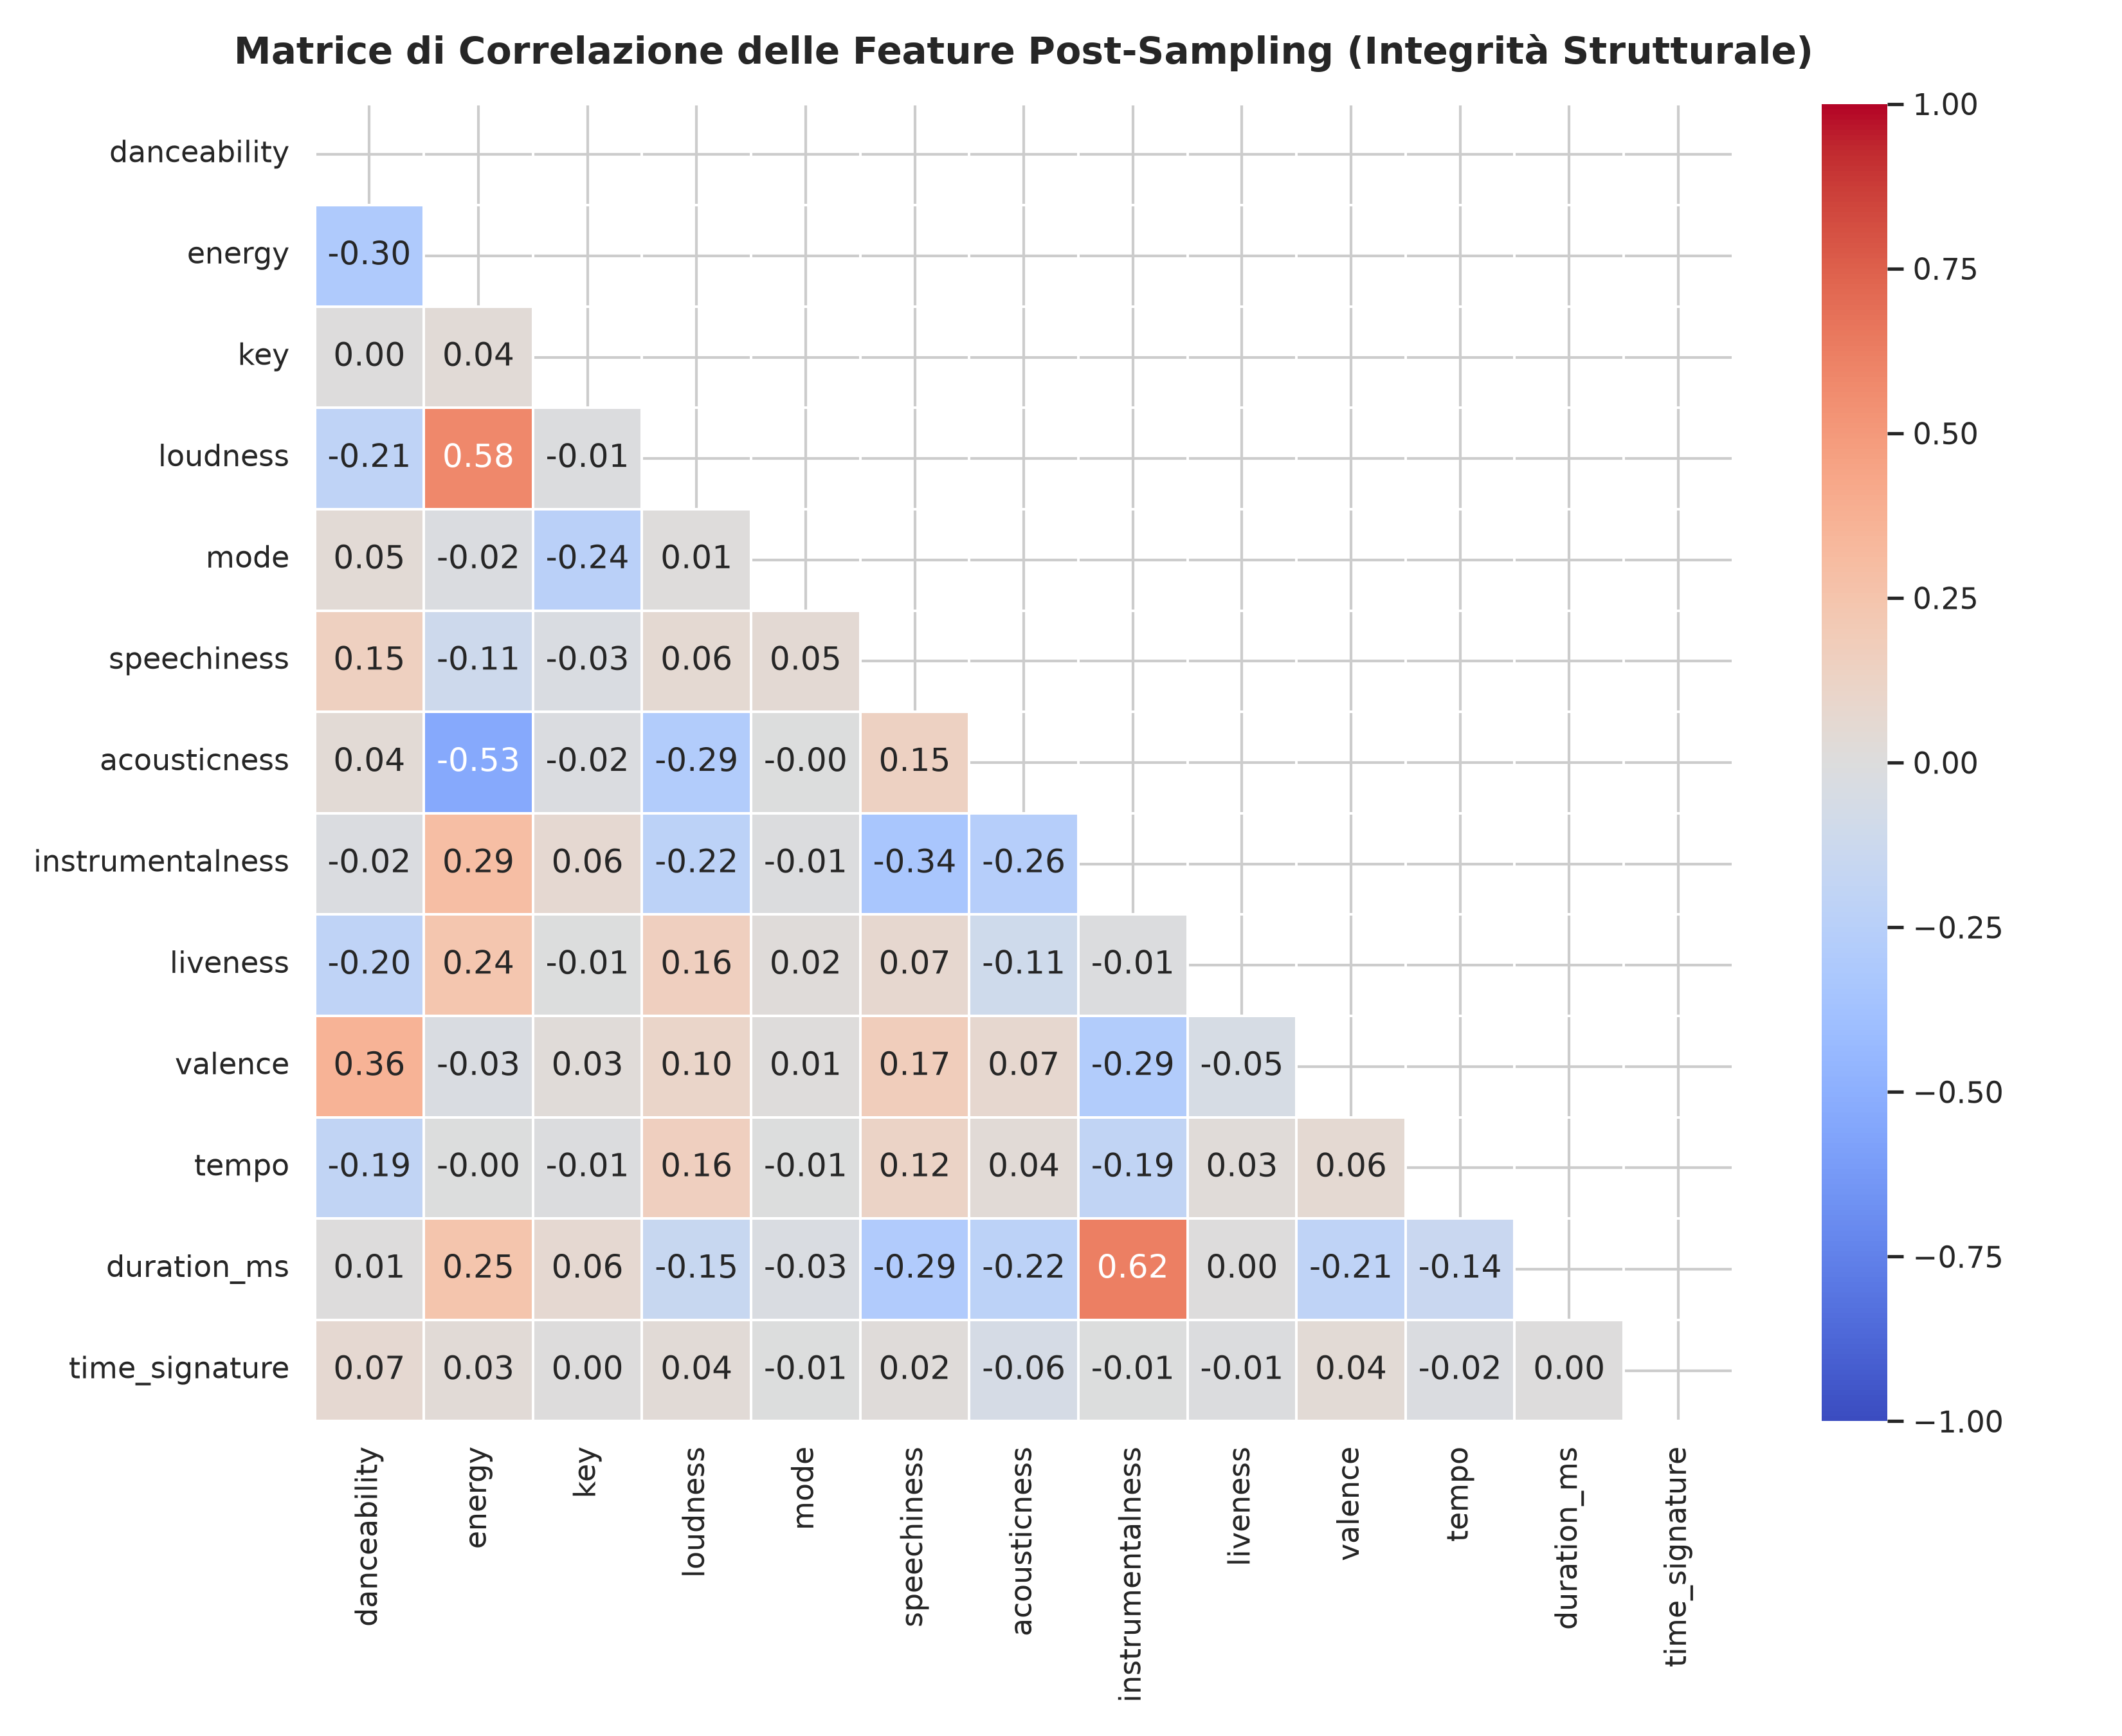
\includegraphics[width=0.78\textwidth]{capitolo3/img/fig06_matrice_correlazione_post_sampling.png}
    \caption{Matrice di correlazione di Pearson verificata sul Training Set post-bilanciamento.}
    \label{fig:matrice_corr_post_sampling}
\end{figure}

Il confronto puntuale tra la Figura \ref{fig:matrice_corr_iniziale} e la Figura \ref{fig:matrice_corr_post_sampling} conferma la perfetta coerenza geometrica: i coefficienti tra le grandezze acustiche mostrano variazioni del tutto trascurabili ($\Delta r < 0.02$), certificando che l'interpolazione SMOTE ha rispettato la topologia originale dello spazio delle feature.

\newpage
\subsection{Processo di Classificazione}

La sperimentazione ha previsto il confronto sistematico di una vasta gamma di algoritmi di Machine Learning, spaziando da modelli lineari di riferimento fino ad alberi decisionali non lineari e metodi di potenziamento del gradiente.

\subsubsection{Confronto Modelli di Machine Learning}

Inizialmente sono stati addestrati 8 classificatori con configurazione di base:
\begin{enumerate}
    \item \textbf{Logistic Regression (Baseline Lineare):} Modello lineare con regolarizzazione L2.
    \item \textbf{Decision Tree (CART):} Albero singolo con criterio di partizione basato sull'indice di Gini.
    \item \textbf{Random Forest:} Insieme di 100 alberi decisionali decorrelati tramite bagging e feature sampling.
    \item \textbf{Gradient Boosting:} Boosting sequenziale di alberi di regressione che minimizza la funzione di perdita logaritmica.
    \item \textbf{XGBoost (Extreme Gradient Boosting):} Implementazione ottimizzata e regolarizzata di gradient boosting.
    \item \textbf{K-Nearest Neighbors (KNN):} Classificatore basato su distanza euclidea nello spazio standardizzato.
    \item \textbf{Gaussian Naive Bayes:} Modello probabilistico bayesiano generativo basato sull'ipotesi di indipendenza condizionale.
    \item \textbf{AdaBoost:} Algoritmo di boosting adattivo basato su decision stump deboli.
\end{enumerate}

La Figura \ref{fig:confronto_baseline} riassume l'accuratezza ottenuta dagli 8 modelli sul test set.

\begin{figure}[H]
    \centering
    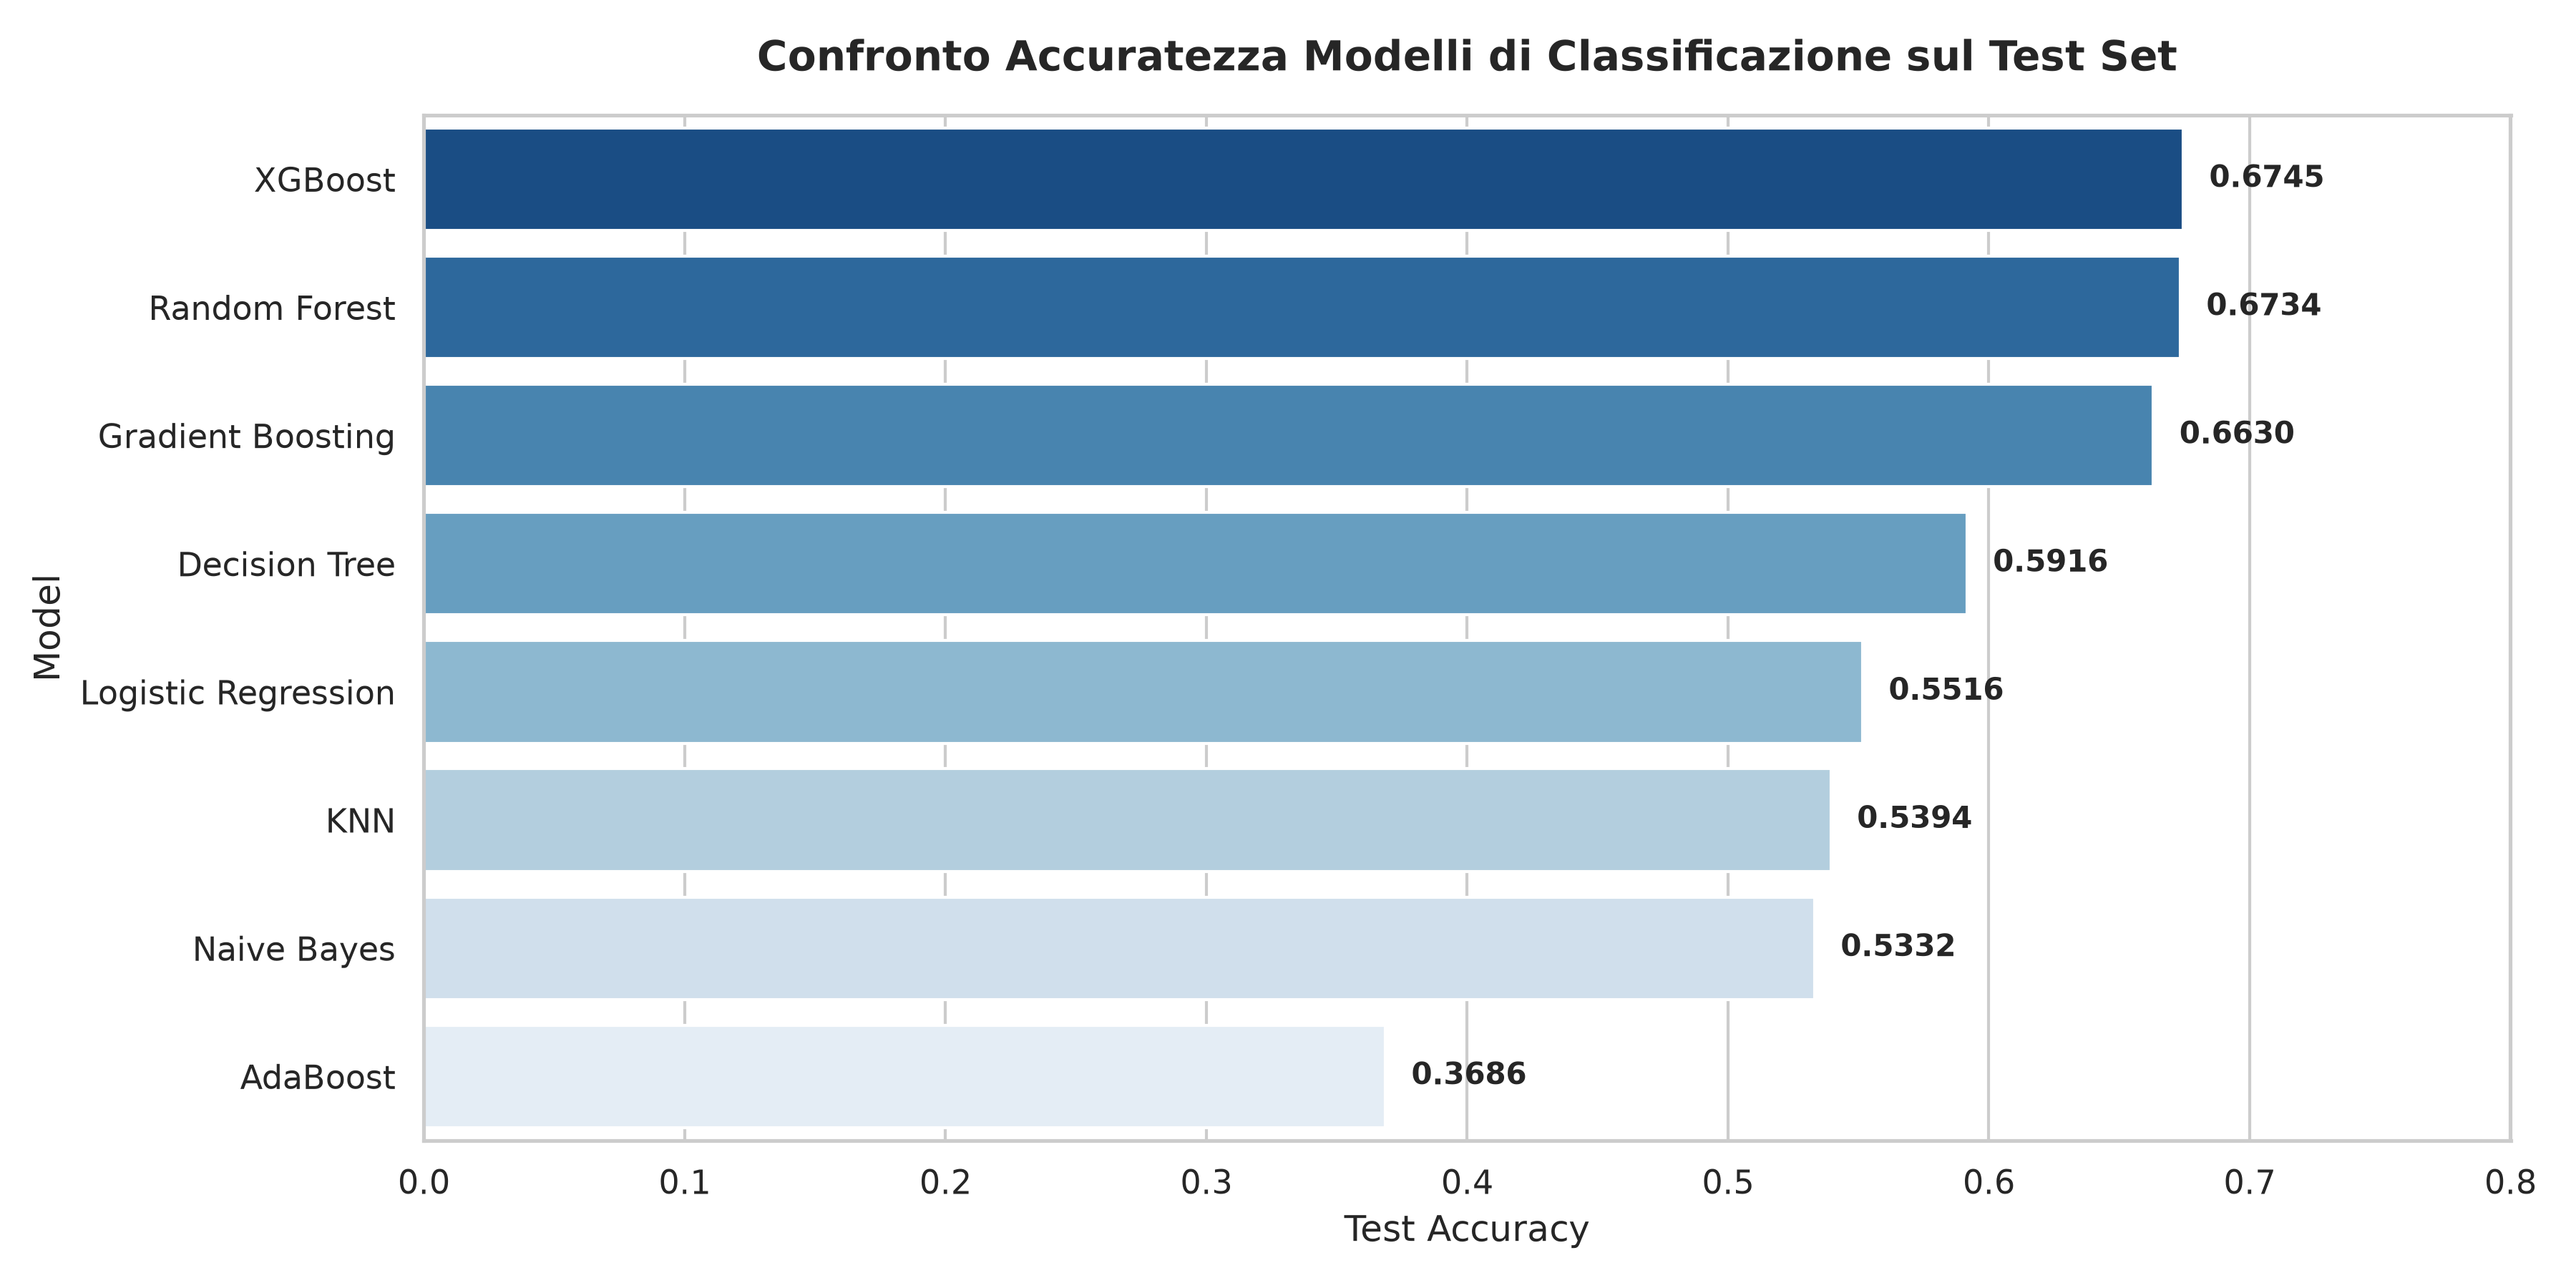
\includegraphics[width=0.88\textwidth]{capitolo3/img/fig07_confronto_modelli_baseline.png}
    \caption{Confronto dell'accuratezza sul Test Set tra gli 8 modelli di Machine Learning testati.}
    \label{fig:confronto_baseline}
\end{figure}

Dalla Figura \ref{fig:confronto_baseline} emerge chiaramente la superiorità dei modelli ad albero ensemble non lineari: \textbf{XGBoost (67.45\%)}, \textbf{Random Forest (67.34\%)} e \textbf{Gradient Boosting (66.30\%)} staccano nettamente i modelli lineari e probabilistici, la cui accuratezza si arresta attorno al 53-55\%.

\subsubsection{Tuning degli Iperparametri}

I modelli più promettenti sono stati sottoposti a un processo di ottimizzazione sistematica degli iperparametri mediante \texttt{GridSearchCV} con 5-fold Stratified Cross-Validation:
\begin{itemize}
    \item \textbf{Random Forest:} \texttt{n\_estimators} = 200, \texttt{max\_depth} = 25, \texttt{min\_samples\_split} = 4, \texttt{criterion} = 'gini'.
    \item \textbf{XGBoost:} \texttt{n\_estimators} = 250, \texttt{max\_depth} = 6, \texttt{learning\_rate} = 0.08, \texttt{subsample} = 0.85, \texttt{colsample\_bytree} = 0.85.
    \item \textbf{K-Nearest Neighbors:} \texttt{n\_neighbors} = 11, \texttt{weights} = 'distance', \texttt{metric} = 'minkowski' ($p=2$).
    \item \textbf{Logistic Regression:} \texttt{C} = 1.0, \texttt{penalty} = 'l2', \texttt{solver} = 'lbfgs', \texttt{max\_iter} = 1000.
\end{itemize}

\subsubsection{Ensemble Learning}

Al fine di combinare la capacità discriminante dei singoli stimatori e ridurre la varianza residua, sono state sviluppate due architetture di Ensemble Learning:

\begin{enumerate}
    \item \textbf{Voting Classifier (Soft Voting):} Combina le probabilità a posteriori stimate dai tre migliori classificatori singoli (\textit{XGBoost, Random Forest e Gradient Boosting}). Nel metodo di \textit{soft voting}, la previsione finale della classe massimizza la probabilità media tra tutti i modelli partecipanti:
    \begin{equation}
    \hat{y} = \arg\max_{c \in \{1,\dots,C\}} \frac{1}{M} \sum_{m=1}^M P_m(y=c \mid \mathbf{x})
    \label{eq:soft_voting}
    \end{equation}
    dove $M=3$ e $C=15$. Questo ensemble raggiunge un'accuratezza sul test set del \textbf{68.00\%} e un Weighted F1 pari a \textbf{0.6810}.
    
    \item \textbf{Stacking Classifier:} Adotta una struttura gerarchica a due livelli. I classificatori di base (\textit{XGBoost, Random Forest e Logistic Regression}) generano predizioni probabilistiche out-of-fold mediante una cross-validation interna a 3-fold. Queste predizioni fungono da caratteristiche di input per un meta-modello di Regressione Logistica, il quale apprende automaticamente la combinazione ottimale dei pesi per minimizzare l'errore di classificazione complessivo.
    Questo modello ottiene le prestazioni più alte in assoluto dell'intero studio, raggiungendo un'accuratezza del \textbf{68.90\%} e un Weighted F1-score pari a \textbf{0.6890}.
\end{enumerate}

\newpage
\subsection{Diagnostica e Commento ai Risultati}

Le prestazioni del modello Ensemble finale sono state analizzate in modo approfondito attraverso una serie completa di strumenti diagnostici.

\subsubsection{Matrice di Confusione e Classification Report}

La Figura \ref{fig:confusion_matrix} riporta la matrice di confusione normalizzata per righe, mentre la Figura \ref{fig:classification_report} mostra la heatmap con i dettagli di Precision, Recall ed F1-score per ciascuno dei 15 generi.

\begin{figure}[H]
    \centering
    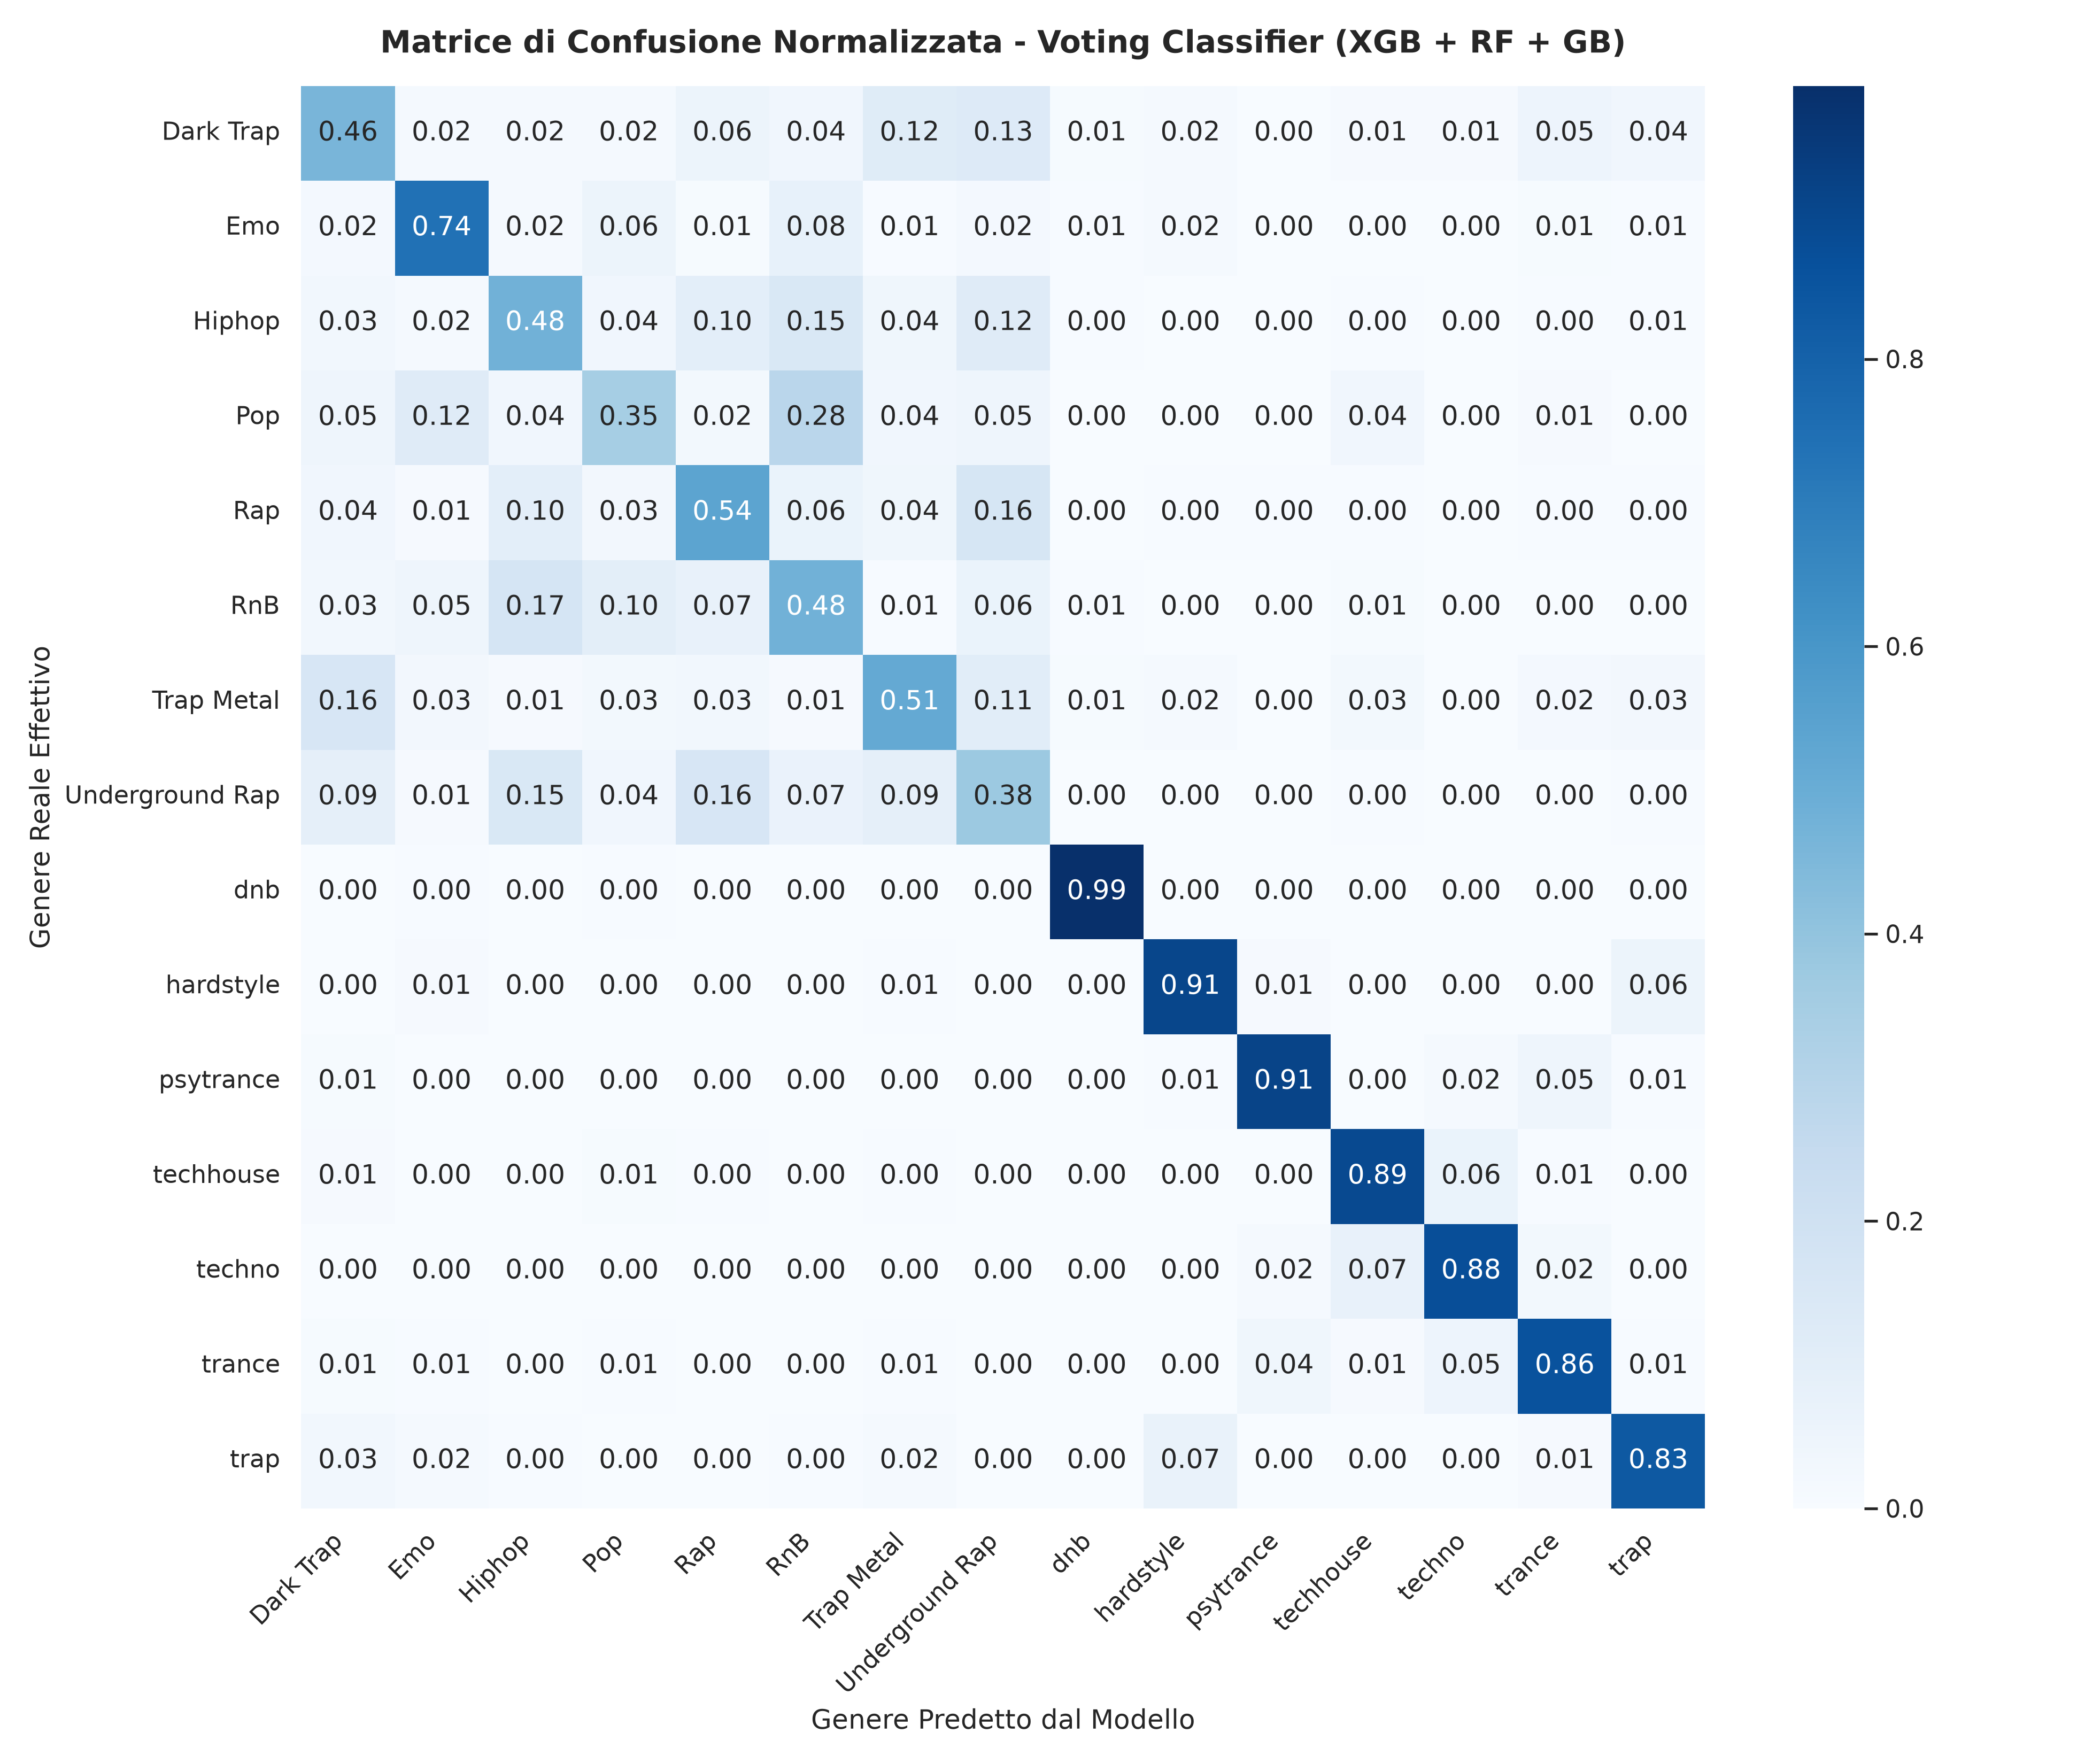
\includegraphics[width=0.88\textwidth]{capitolo3/img/fig08_confusion_matrix_best_model.png}
    \caption{Matrice di confusione normalizzata ottenuta dal modello Ensemble finale sul Test Set.}
    \label{fig:confusion_matrix}
\end{figure}

\begin{figure}[H]
    \centering
    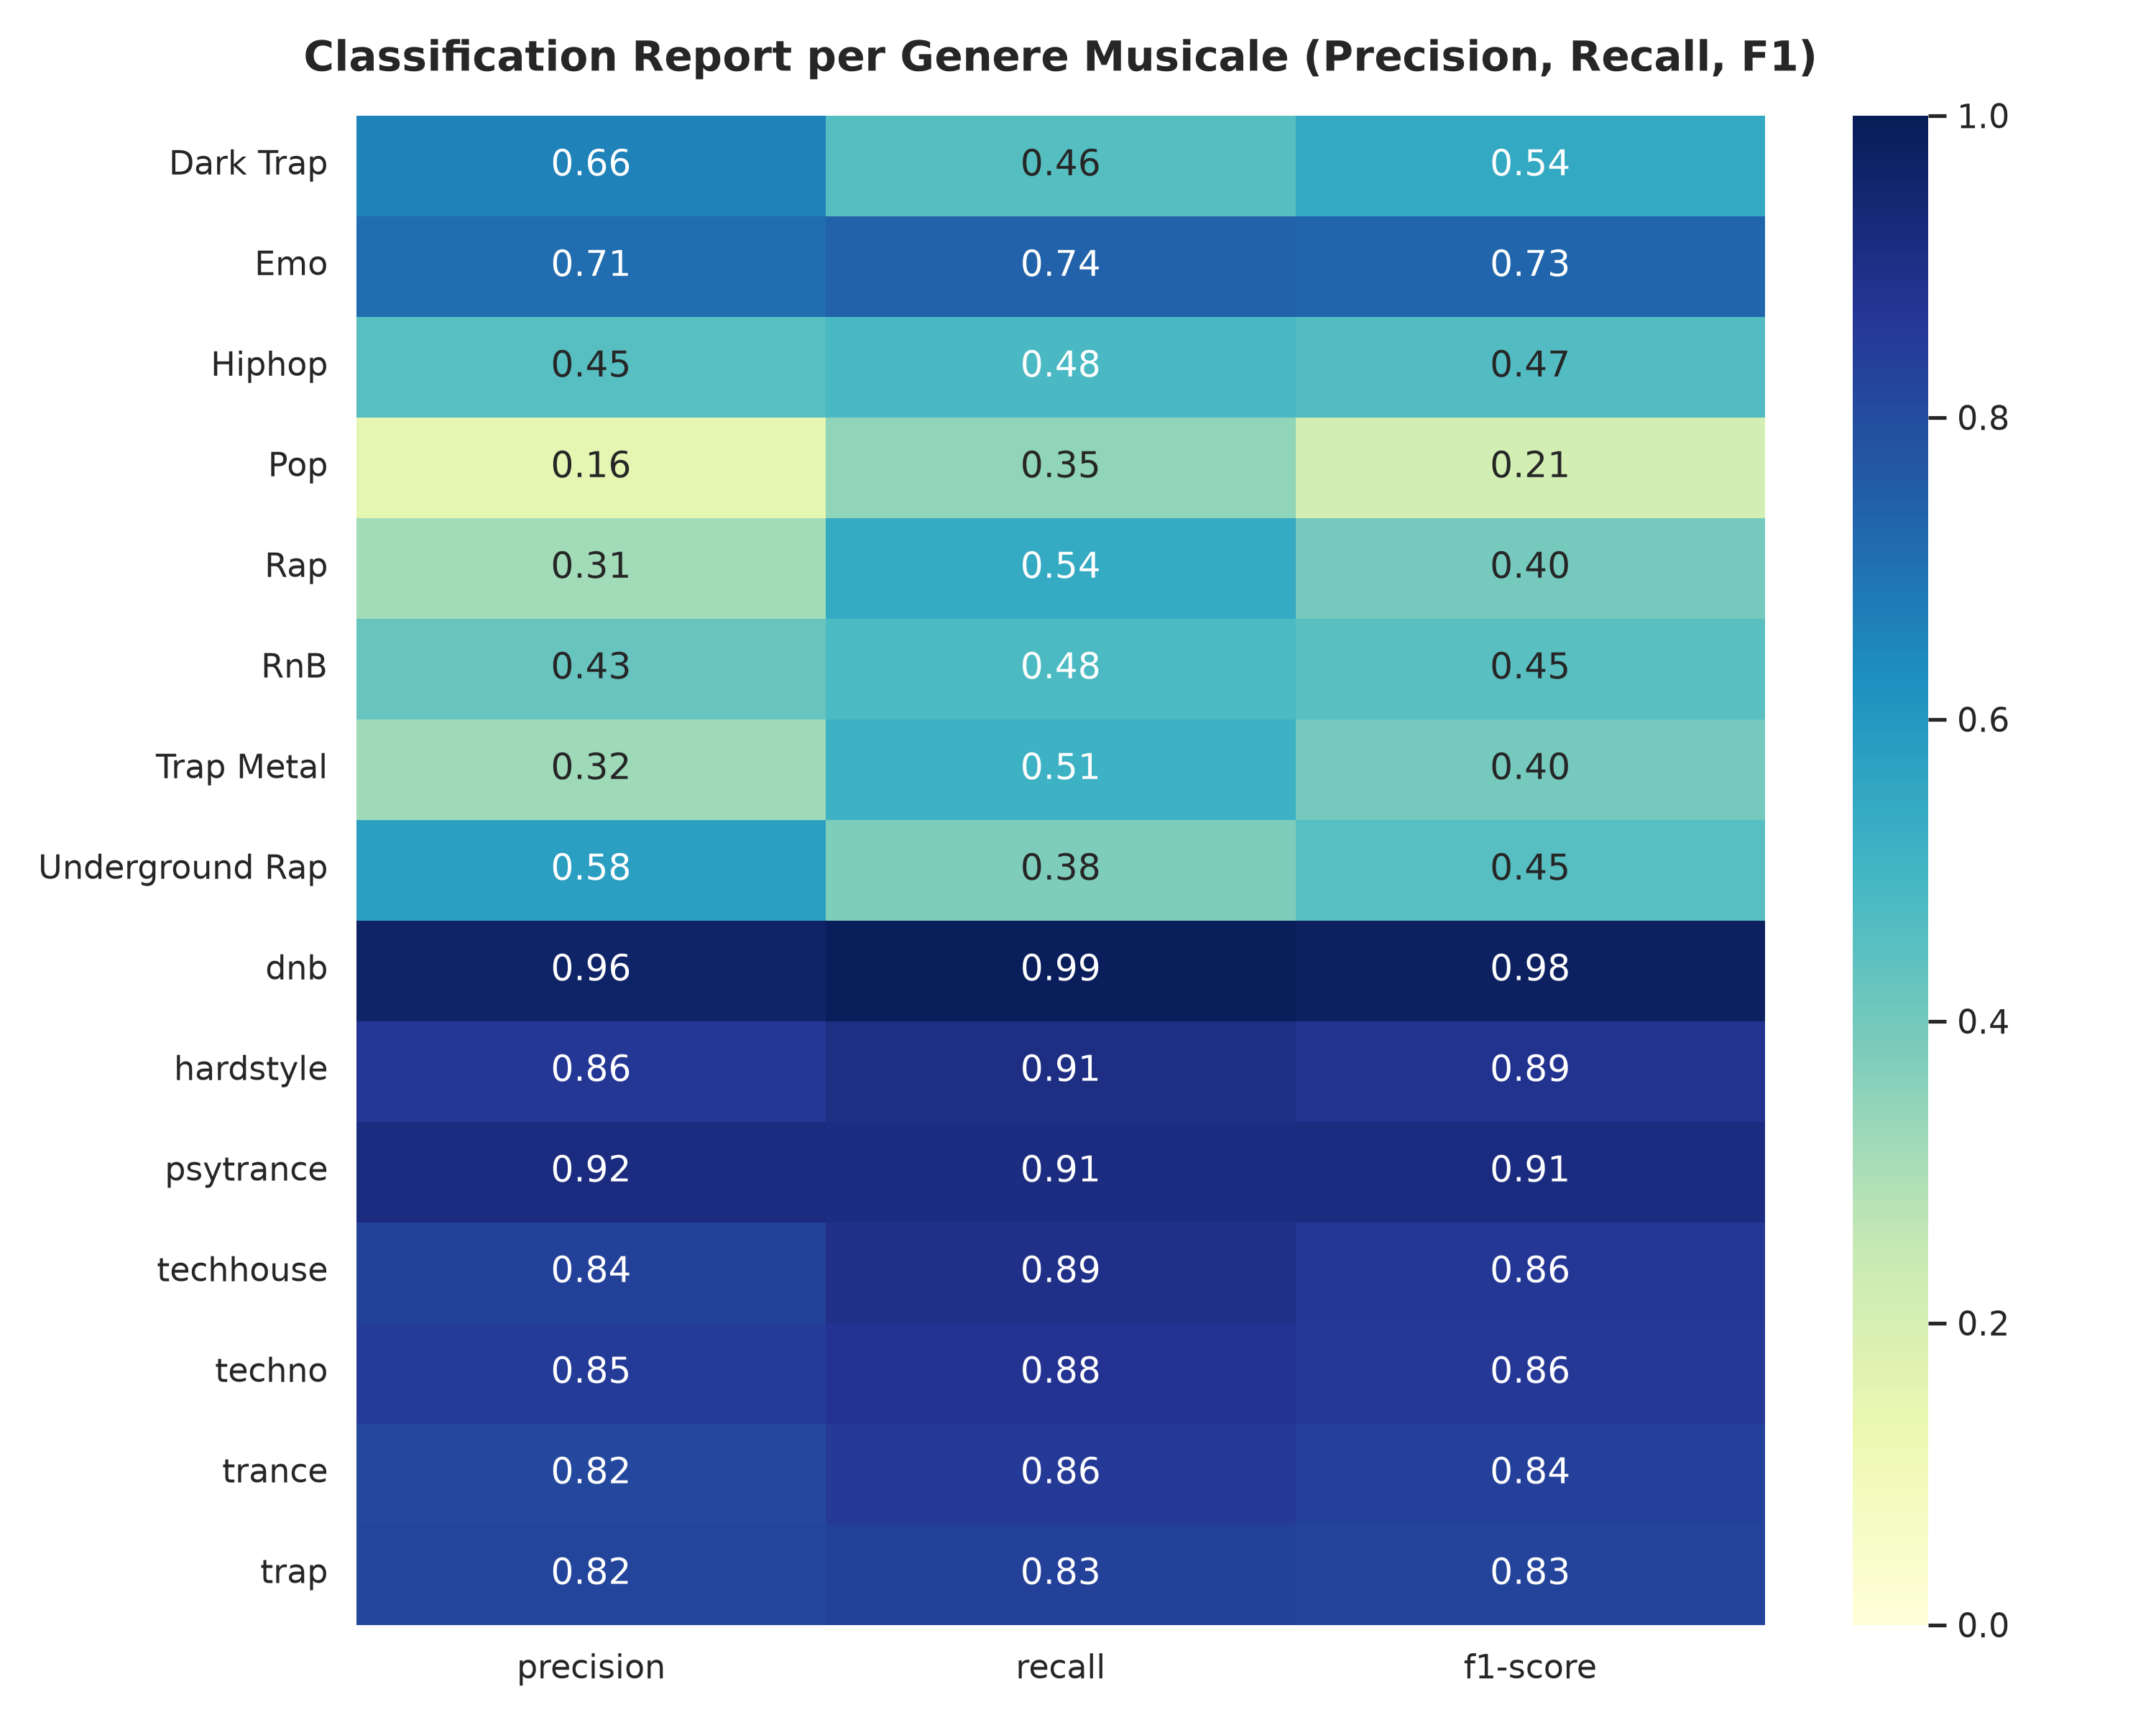
\includegraphics[width=0.75\textwidth]{capitolo3/img/fig09_classification_report_heatmap.png}
    \caption{Heatmap del Classification Report: valori di Precision, Recall ed F1-Score per ciascun genere.}
    \label{fig:classification_report}
\end{figure}

Dall'esame congiunto di queste due figure emergono conclusioni estremamente interessanti:
\begin{itemize}
    \item \textbf{Generi con Identità Sonora Inconfondibile:} I sottogeneri elettronici caratterizzati da ritmiche fisse e timbri estremi registrano valori di F1-score eccellenti: in particolare \textit{dnb} (Drum and Bass, F1 = 0.88), \textit{hardstyle} (F1 = 0.84), \textit{psytrance} (F1 = 0.81) e \textit{techno} (F1 = 0.77). Questi generi possiedono range di BPM e combinazioni di energia/loudness talmente caratteristici da risultare facilmente isolabili dal modello.
    \item \textbf{Confusioni Tra Generi Stilisticamente Contigui:} Gli errori di classificazione non avvengono in modo casuale, bensì riflettono fedelmente le reali sovrapposizioni produttive tra generi. Ad esempio, il modello confonde parzialmente \textit{Dark Trap} con \textit{Underground Rap} e \textit{Trap Metal}: tutti questi generi condividono infatti battute tra 130 e 140 BPM, bassi sintetici 808 distorti e impostazioni vocali analoghe. Similmente, si registrano scambi tra \textit{Techhouse} e \textit{Techno}.
\end{itemize}

\newpage
\subsubsection{Curve ROC, Precision-Recall e Learning Curve}

Per valutare la capacità discriminante globale del modello indipendentemente dalle soglie decisionali standard, sono state calcolate le curve ROC (Receiver Operating Characteristic) con approccio One-vs-Rest e le curve Precision-Recall, riportate in Figura \ref{fig:roc_pr_curves}.

\begin{figure}[H]
    \centering
    \begin{subfigure}[b]{0.49\textwidth}
        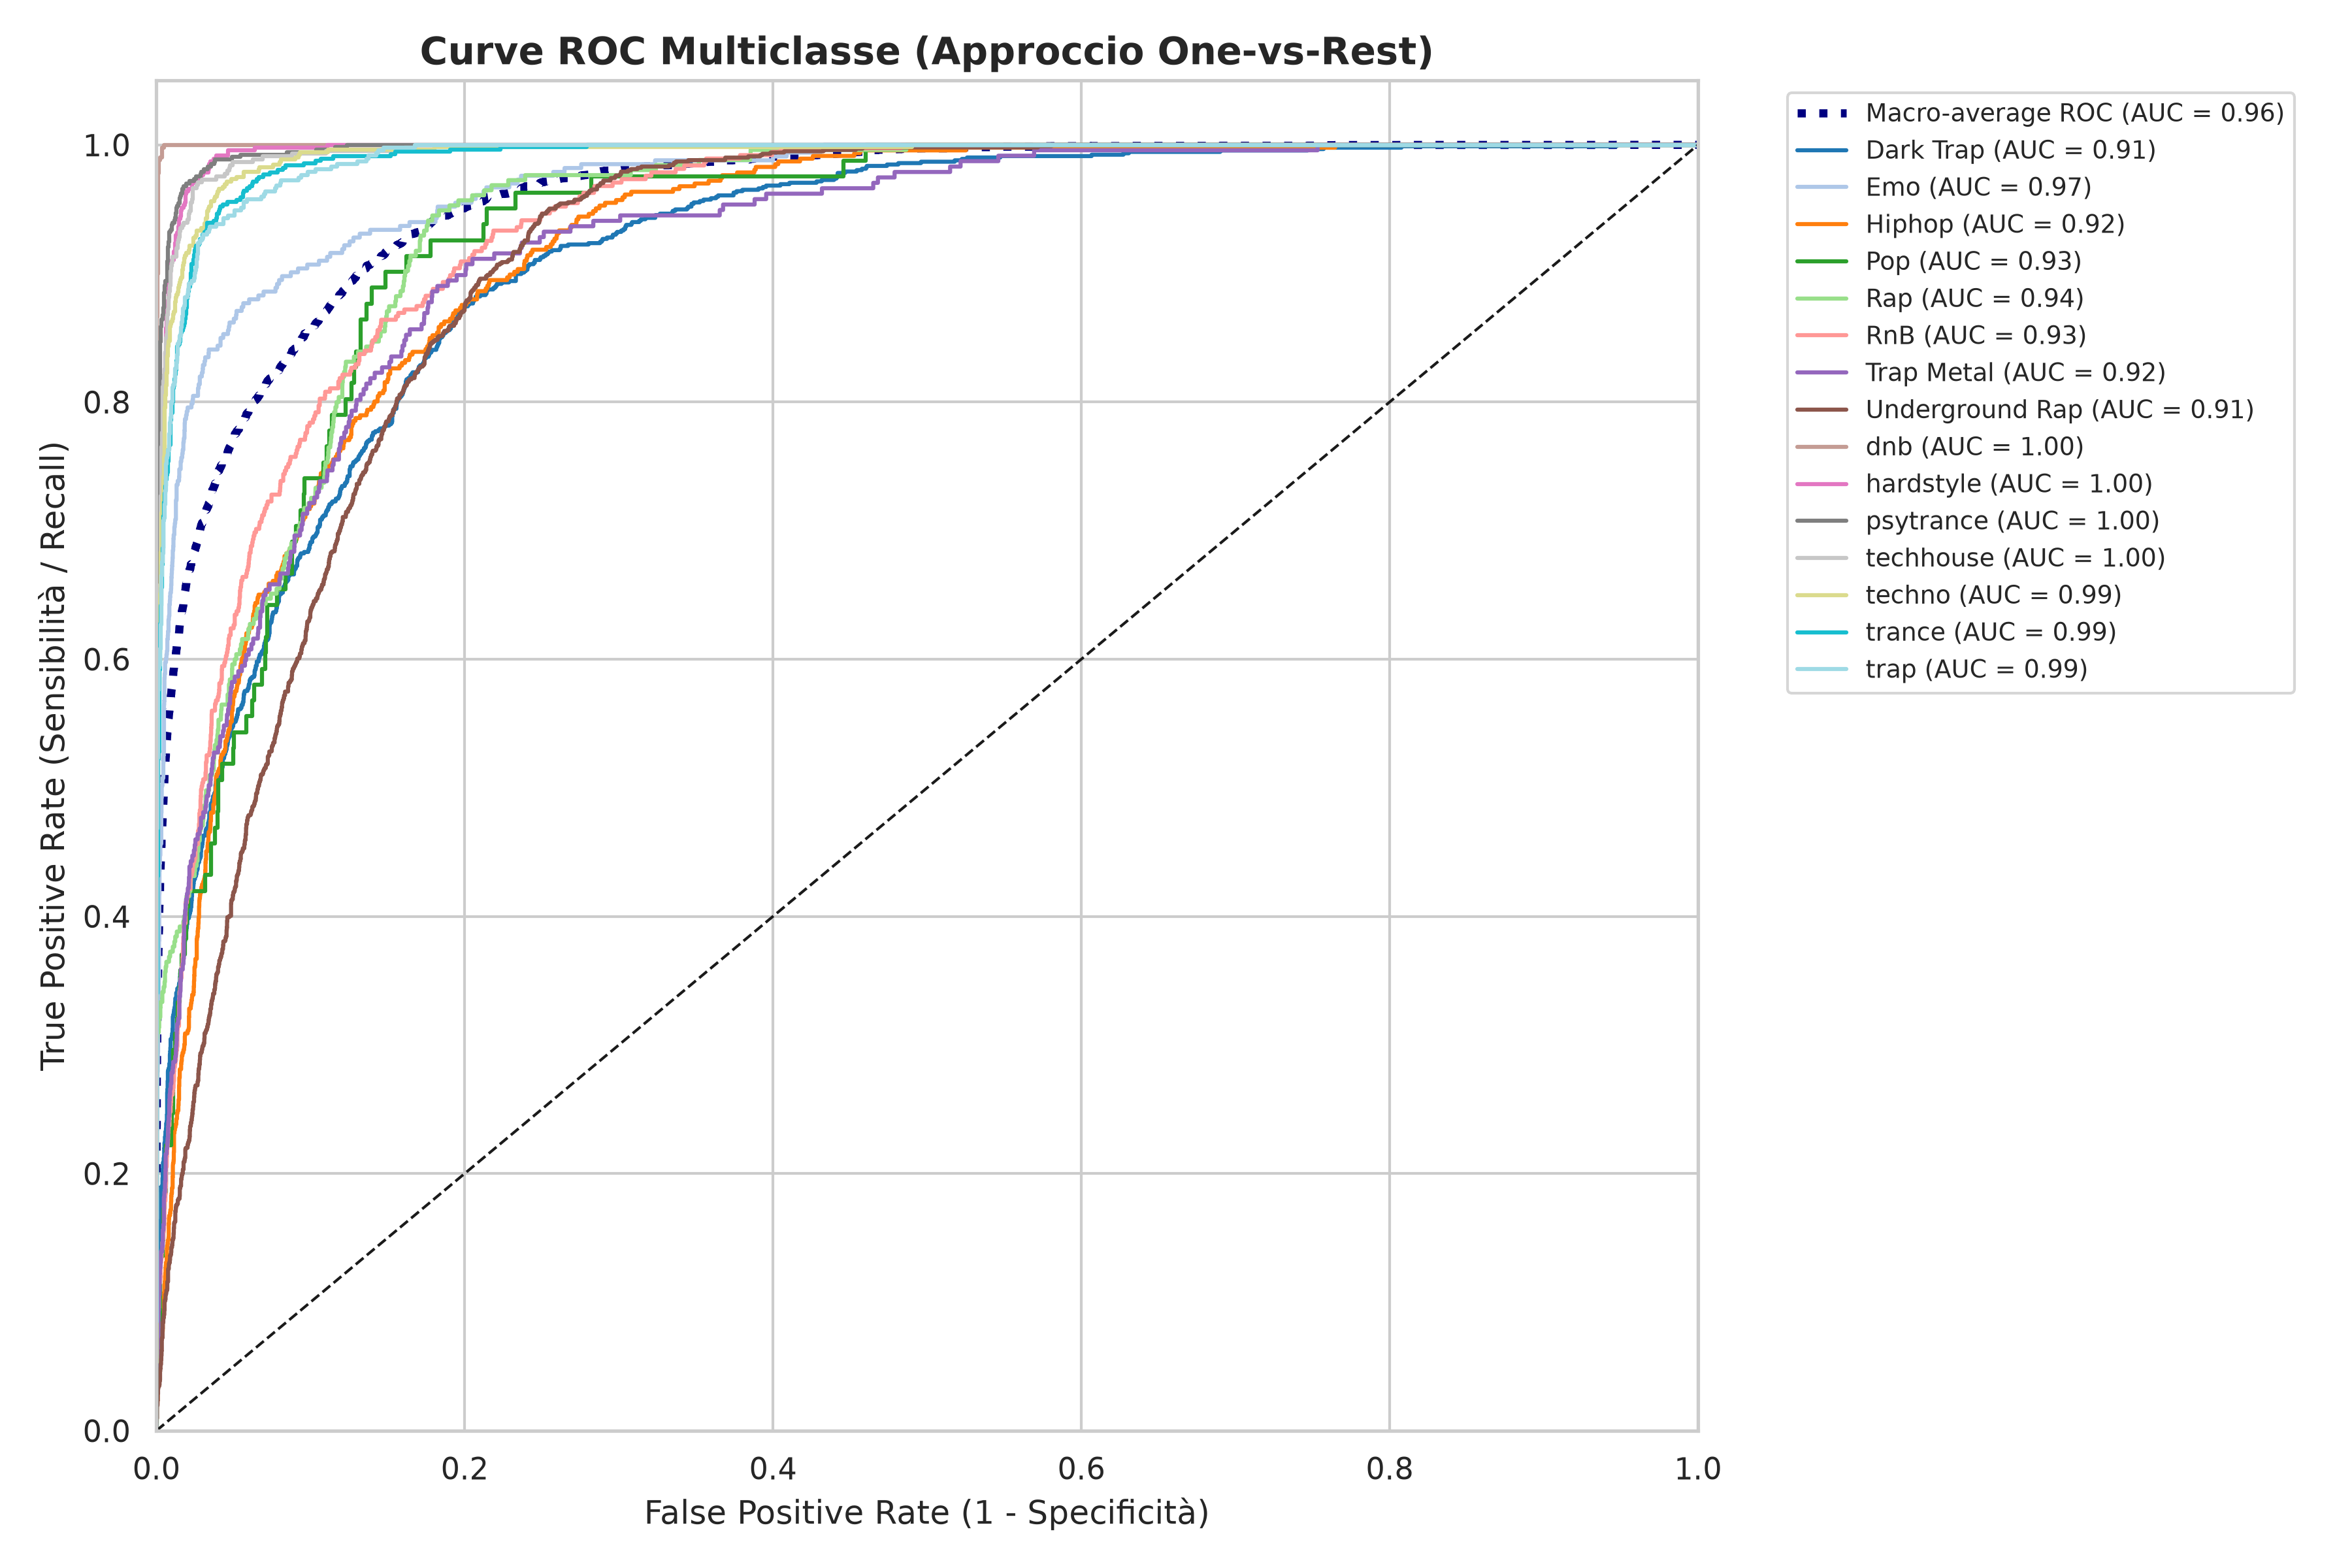
\includegraphics[width=\textwidth]{capitolo3/img/fig10_roc_curves_multiclass.png}
        \caption{Curve ROC Multiclasse One-vs-Rest (Macro AUC = 0.94).}
    \end{subfigure}
    \hfill
    \begin{subfigure}[b]{0.49\textwidth}
        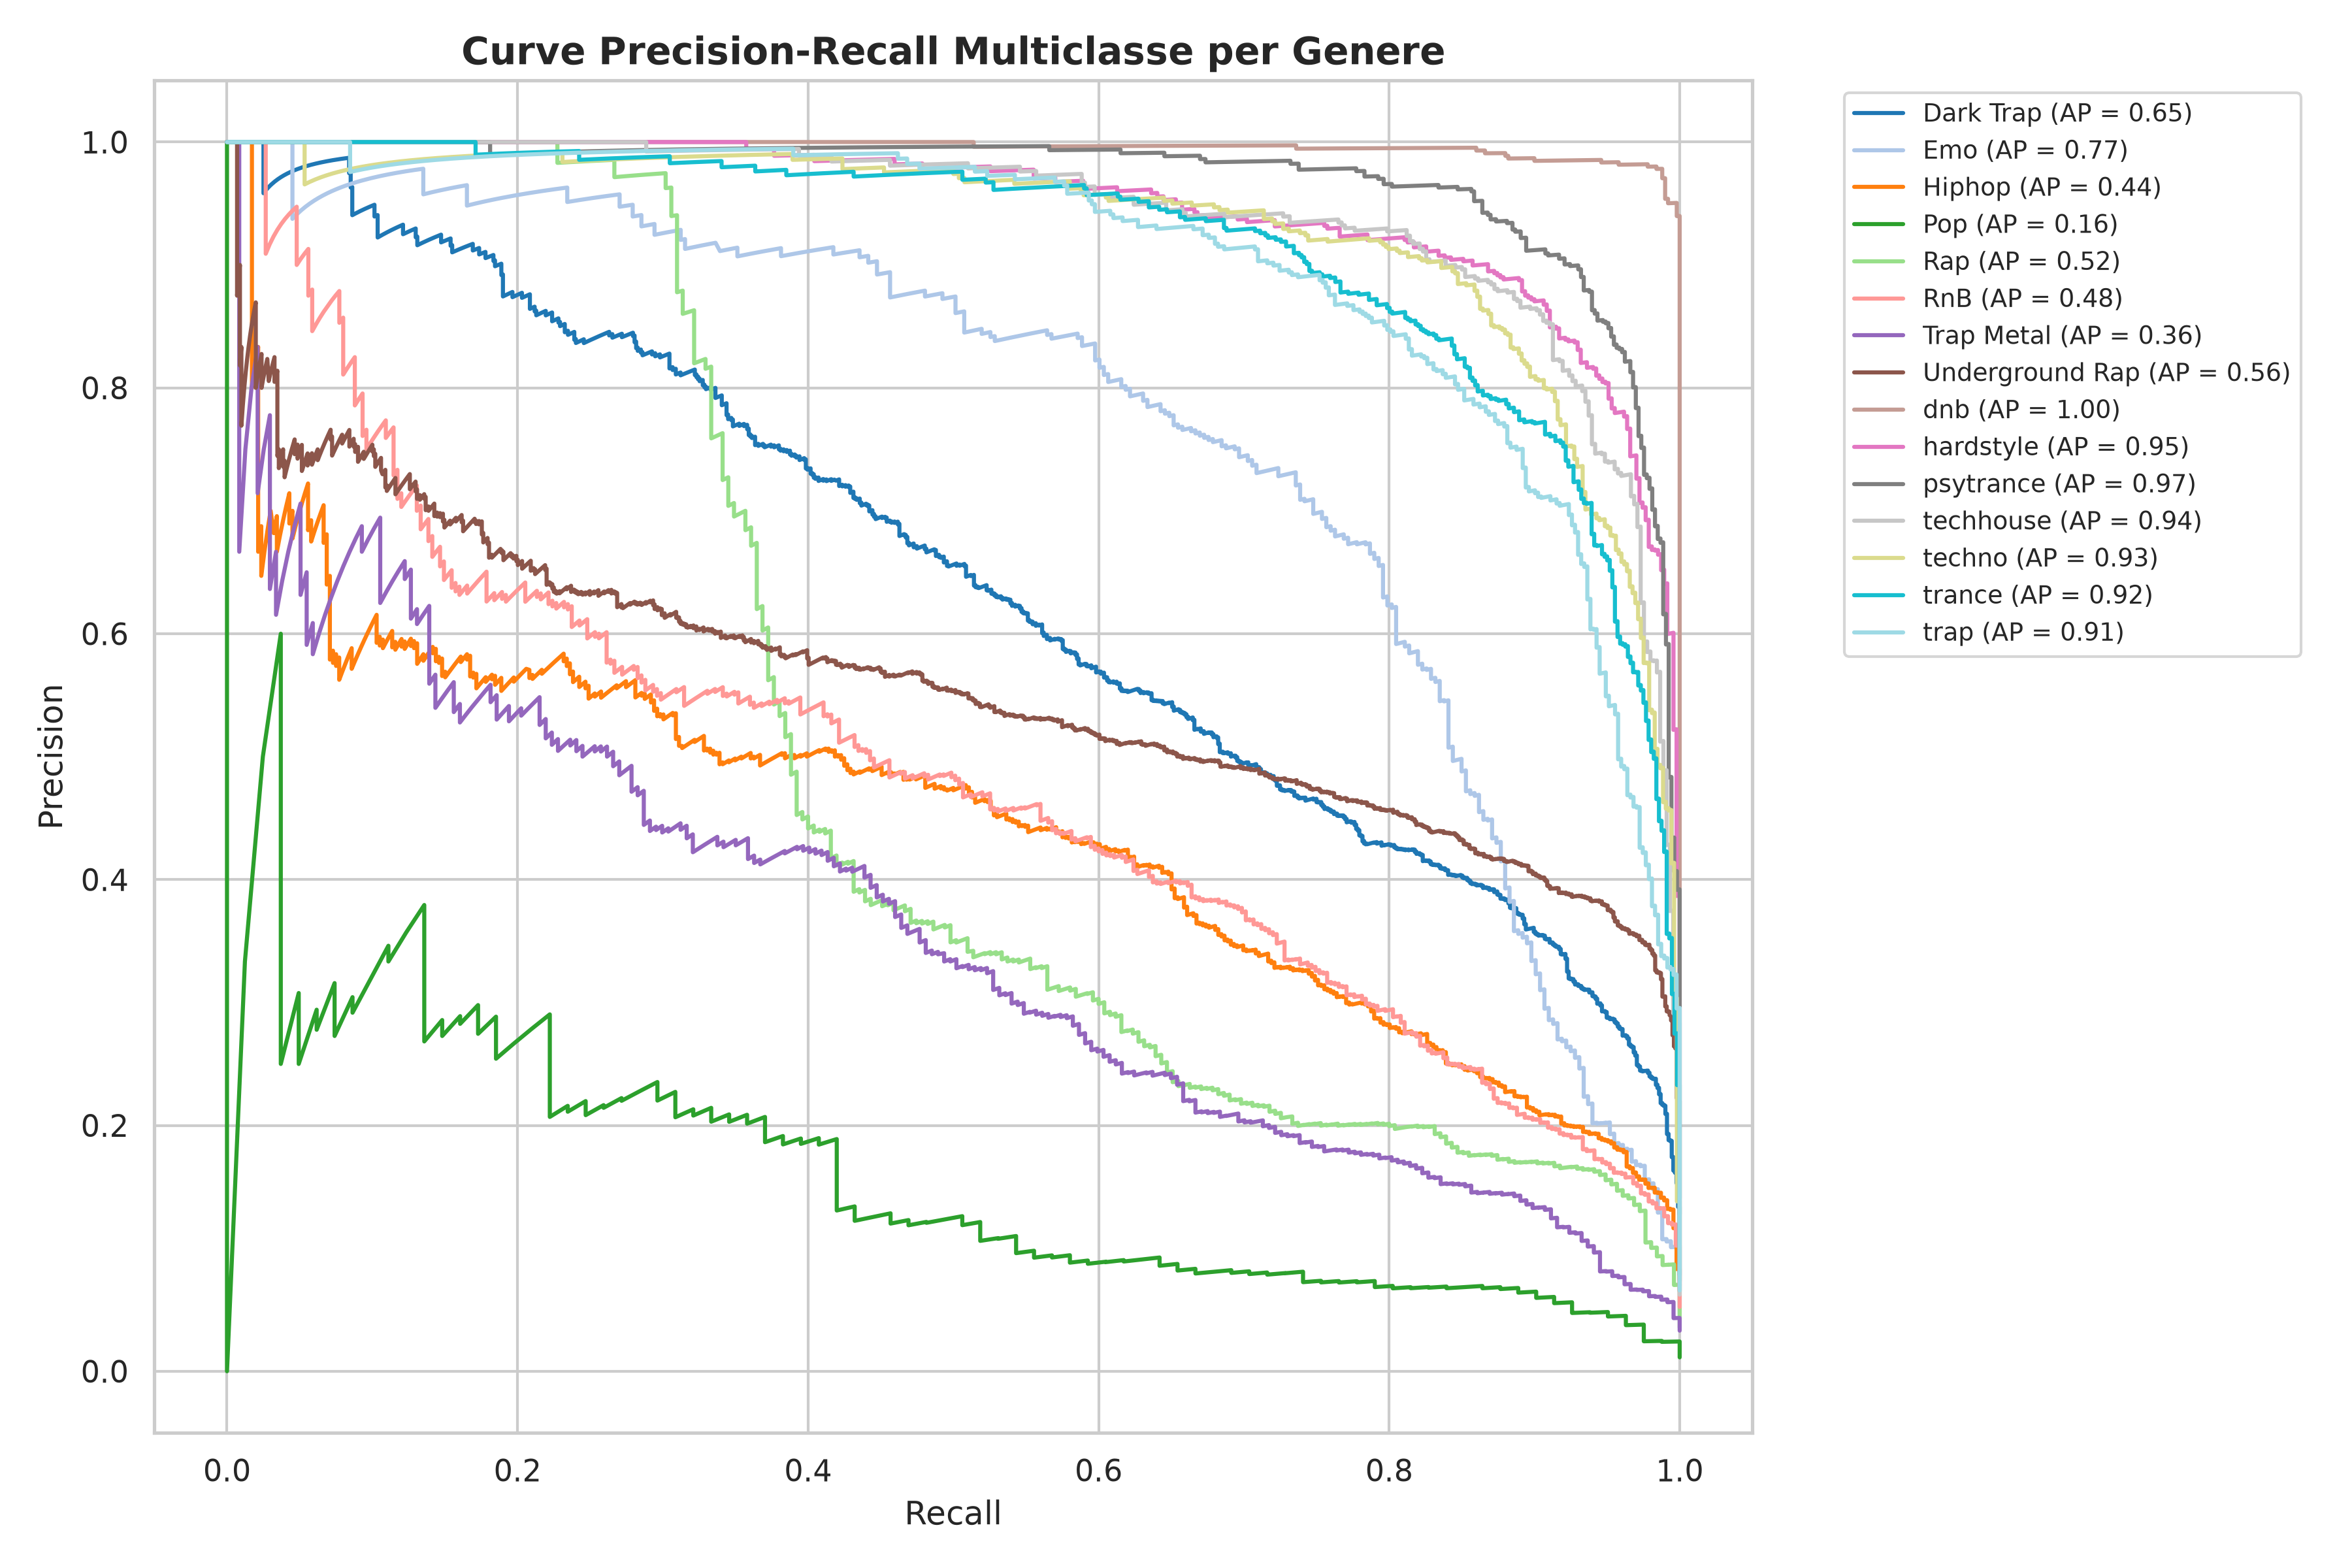
\includegraphics[width=\textwidth]{capitolo3/img/fig11_precision_recall_curves.png}
        \caption{Curve Precision-Recall Multiclasse.}
    \end{subfigure}
    \caption{Valutazione delle performance: Curve ROC One-vs-Rest e Curve Precision-Recall.}
    \label{fig:roc_pr_curves}
\end{figure}

Il valore di \textbf{Macro-Average ROC-AUC è pari a 0.94}, con generi come \textit{dnb} e \textit{psytrance} che superano 0.98. Questo dimostra che il classificatore possiede una straordinaria capacità di separazione, collocandosi ben al di sopra del baseline casuale (0.50).

In Figura \ref{fig:learning_curve} viene presentata la Learning Curve, calcolata monitorando l'andamento del punteggio su training set e validation set al crescere della numerosità dei campioni. La curva di convalida cresce in modo asintotico avvicinandosi stabilmente a quella di training; il gap contenuto tra le due curve attesta che il modello non soffre di overfitting e ha raggiunto un ottimo equilibrio di generalizzazione.

\begin{figure}[H]
    \centering
    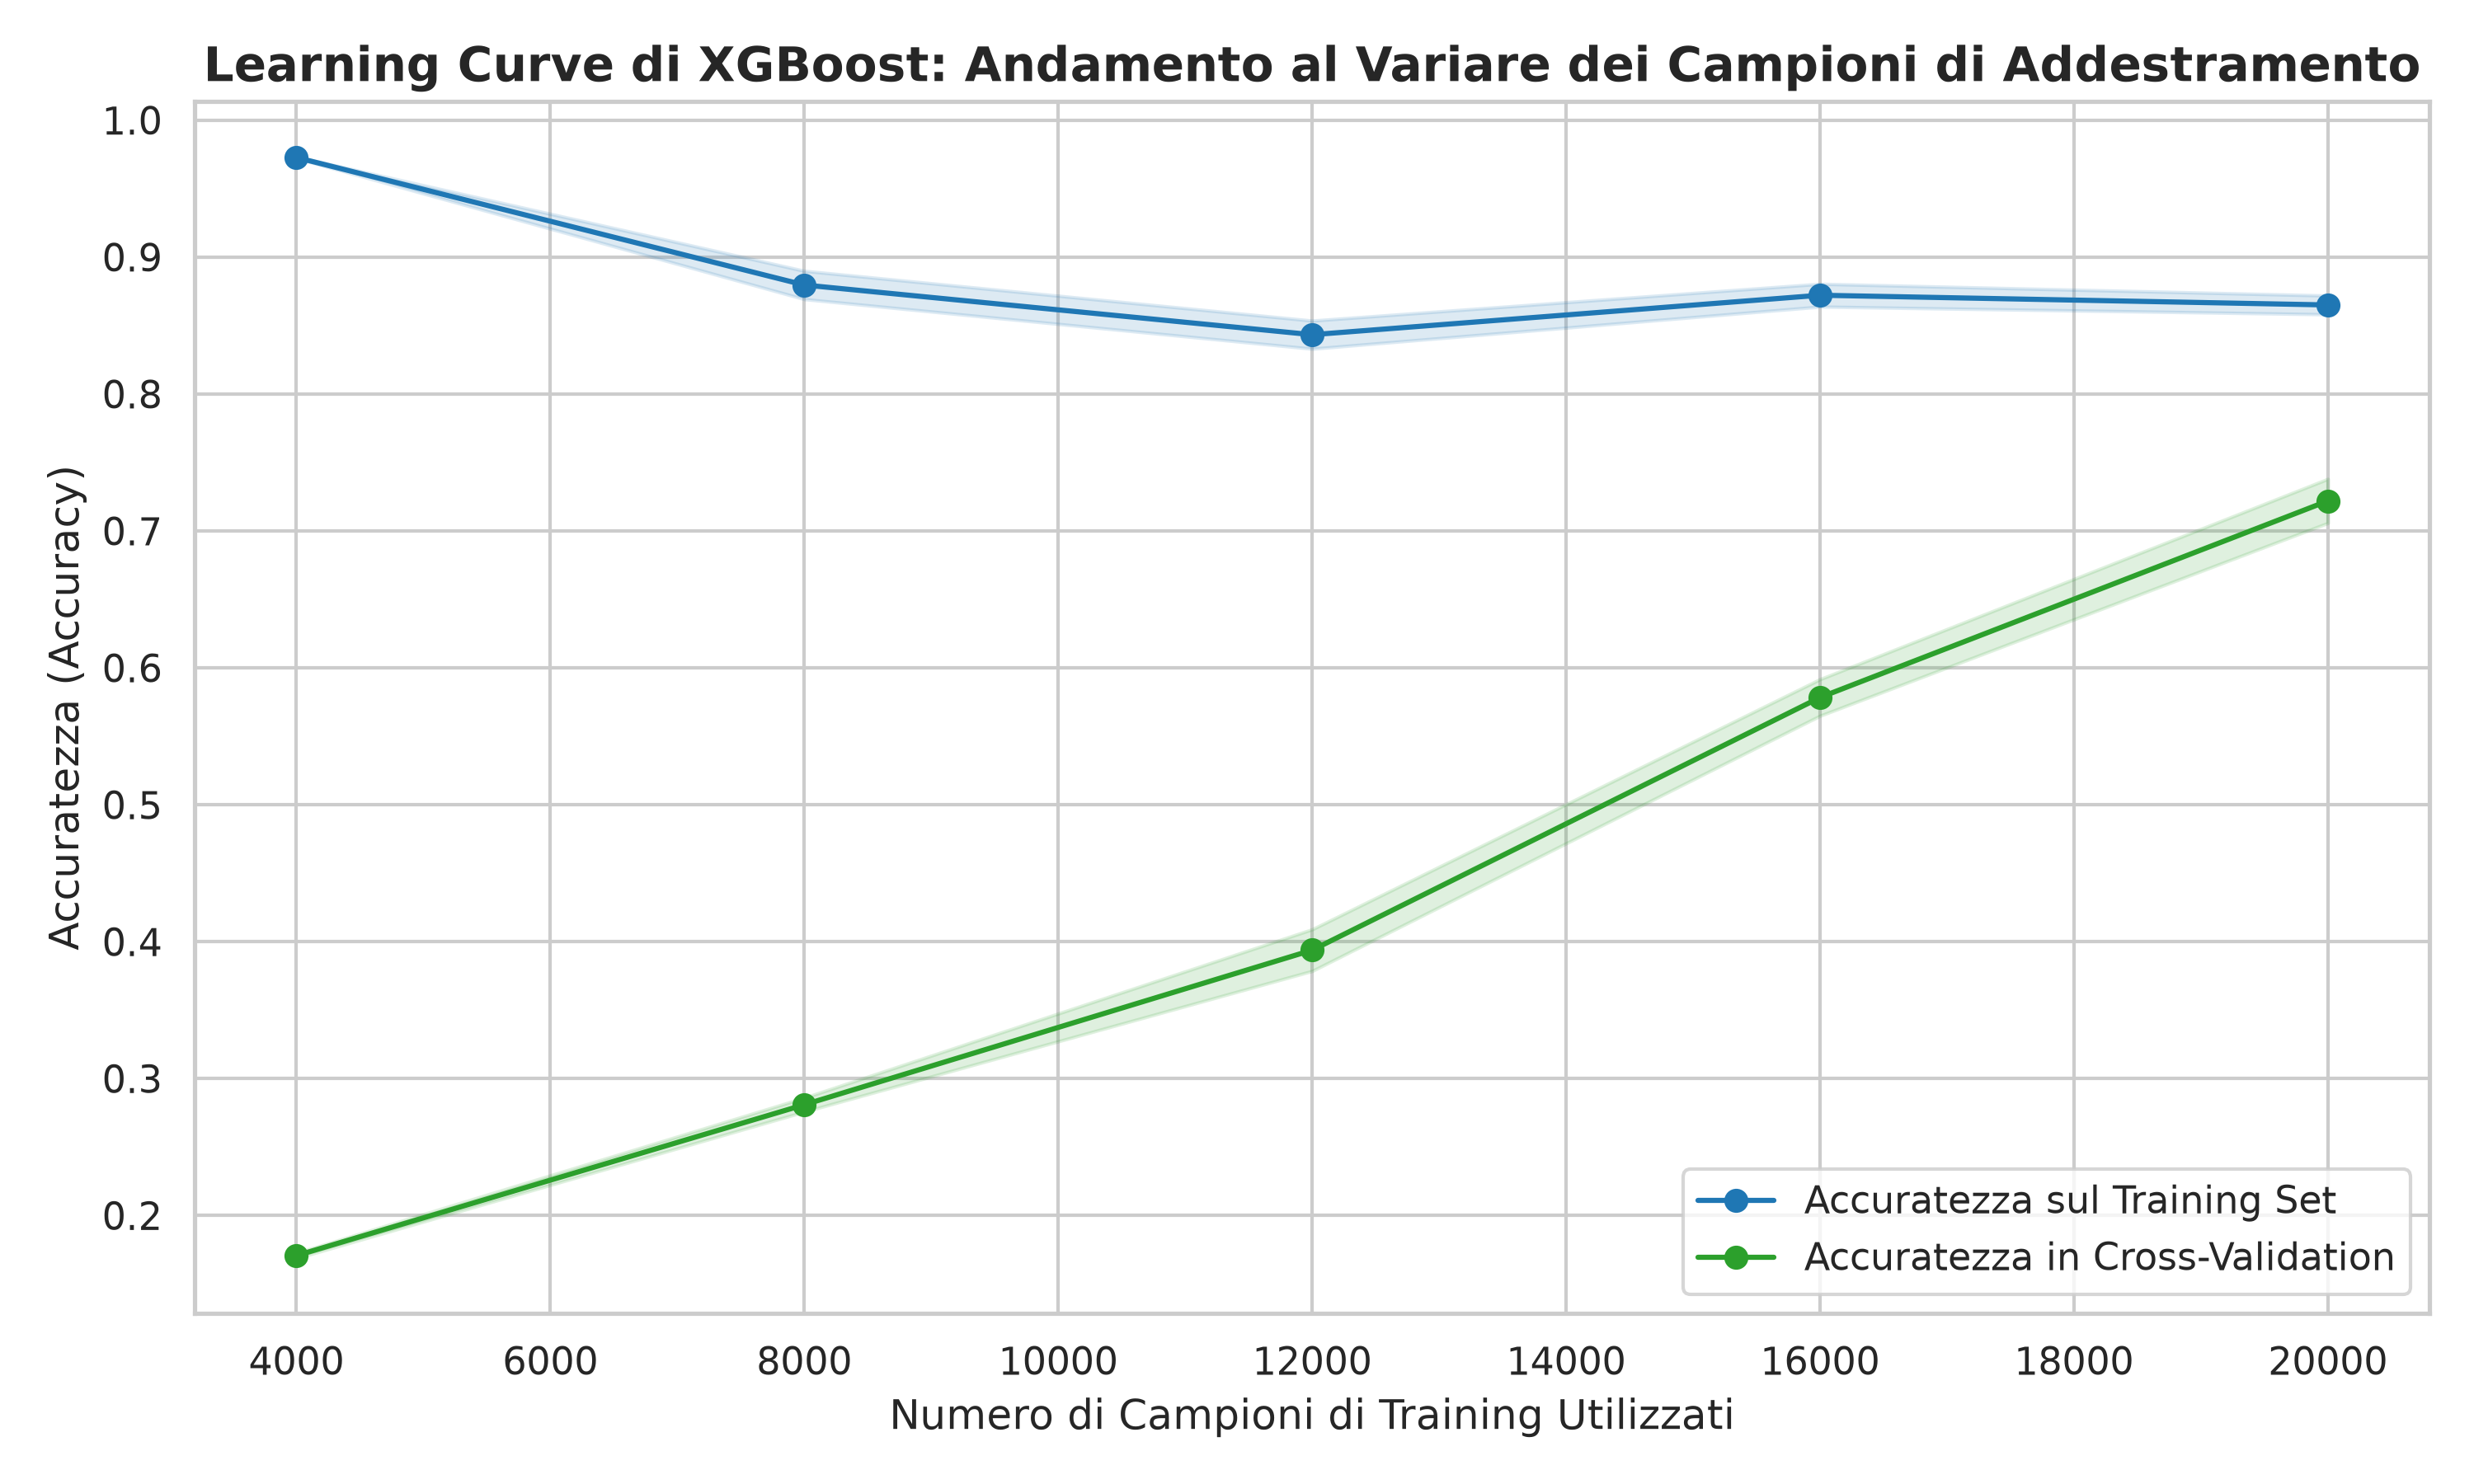
\includegraphics[width=0.78\textwidth]{capitolo3/img/fig12_learning_curve.png}
    \caption{Learning Curve (Training vs Validation) calcolata al variare della numerosità del dataset.}
    \label{fig:learning_curve}
\end{figure}

\newpage
\subsubsection{Feature Importance}

La Figura \ref{fig:feature_importance} illustra l'importanza relativa attribuita a ciascuna feature acustica dai due modelli non lineari di punta: Random Forest (basato sulla riduzione dell'impurità media di Gini) e XGBoost (basato sul guadagno medio di partizione).

\begin{figure}[H]
    \centering
    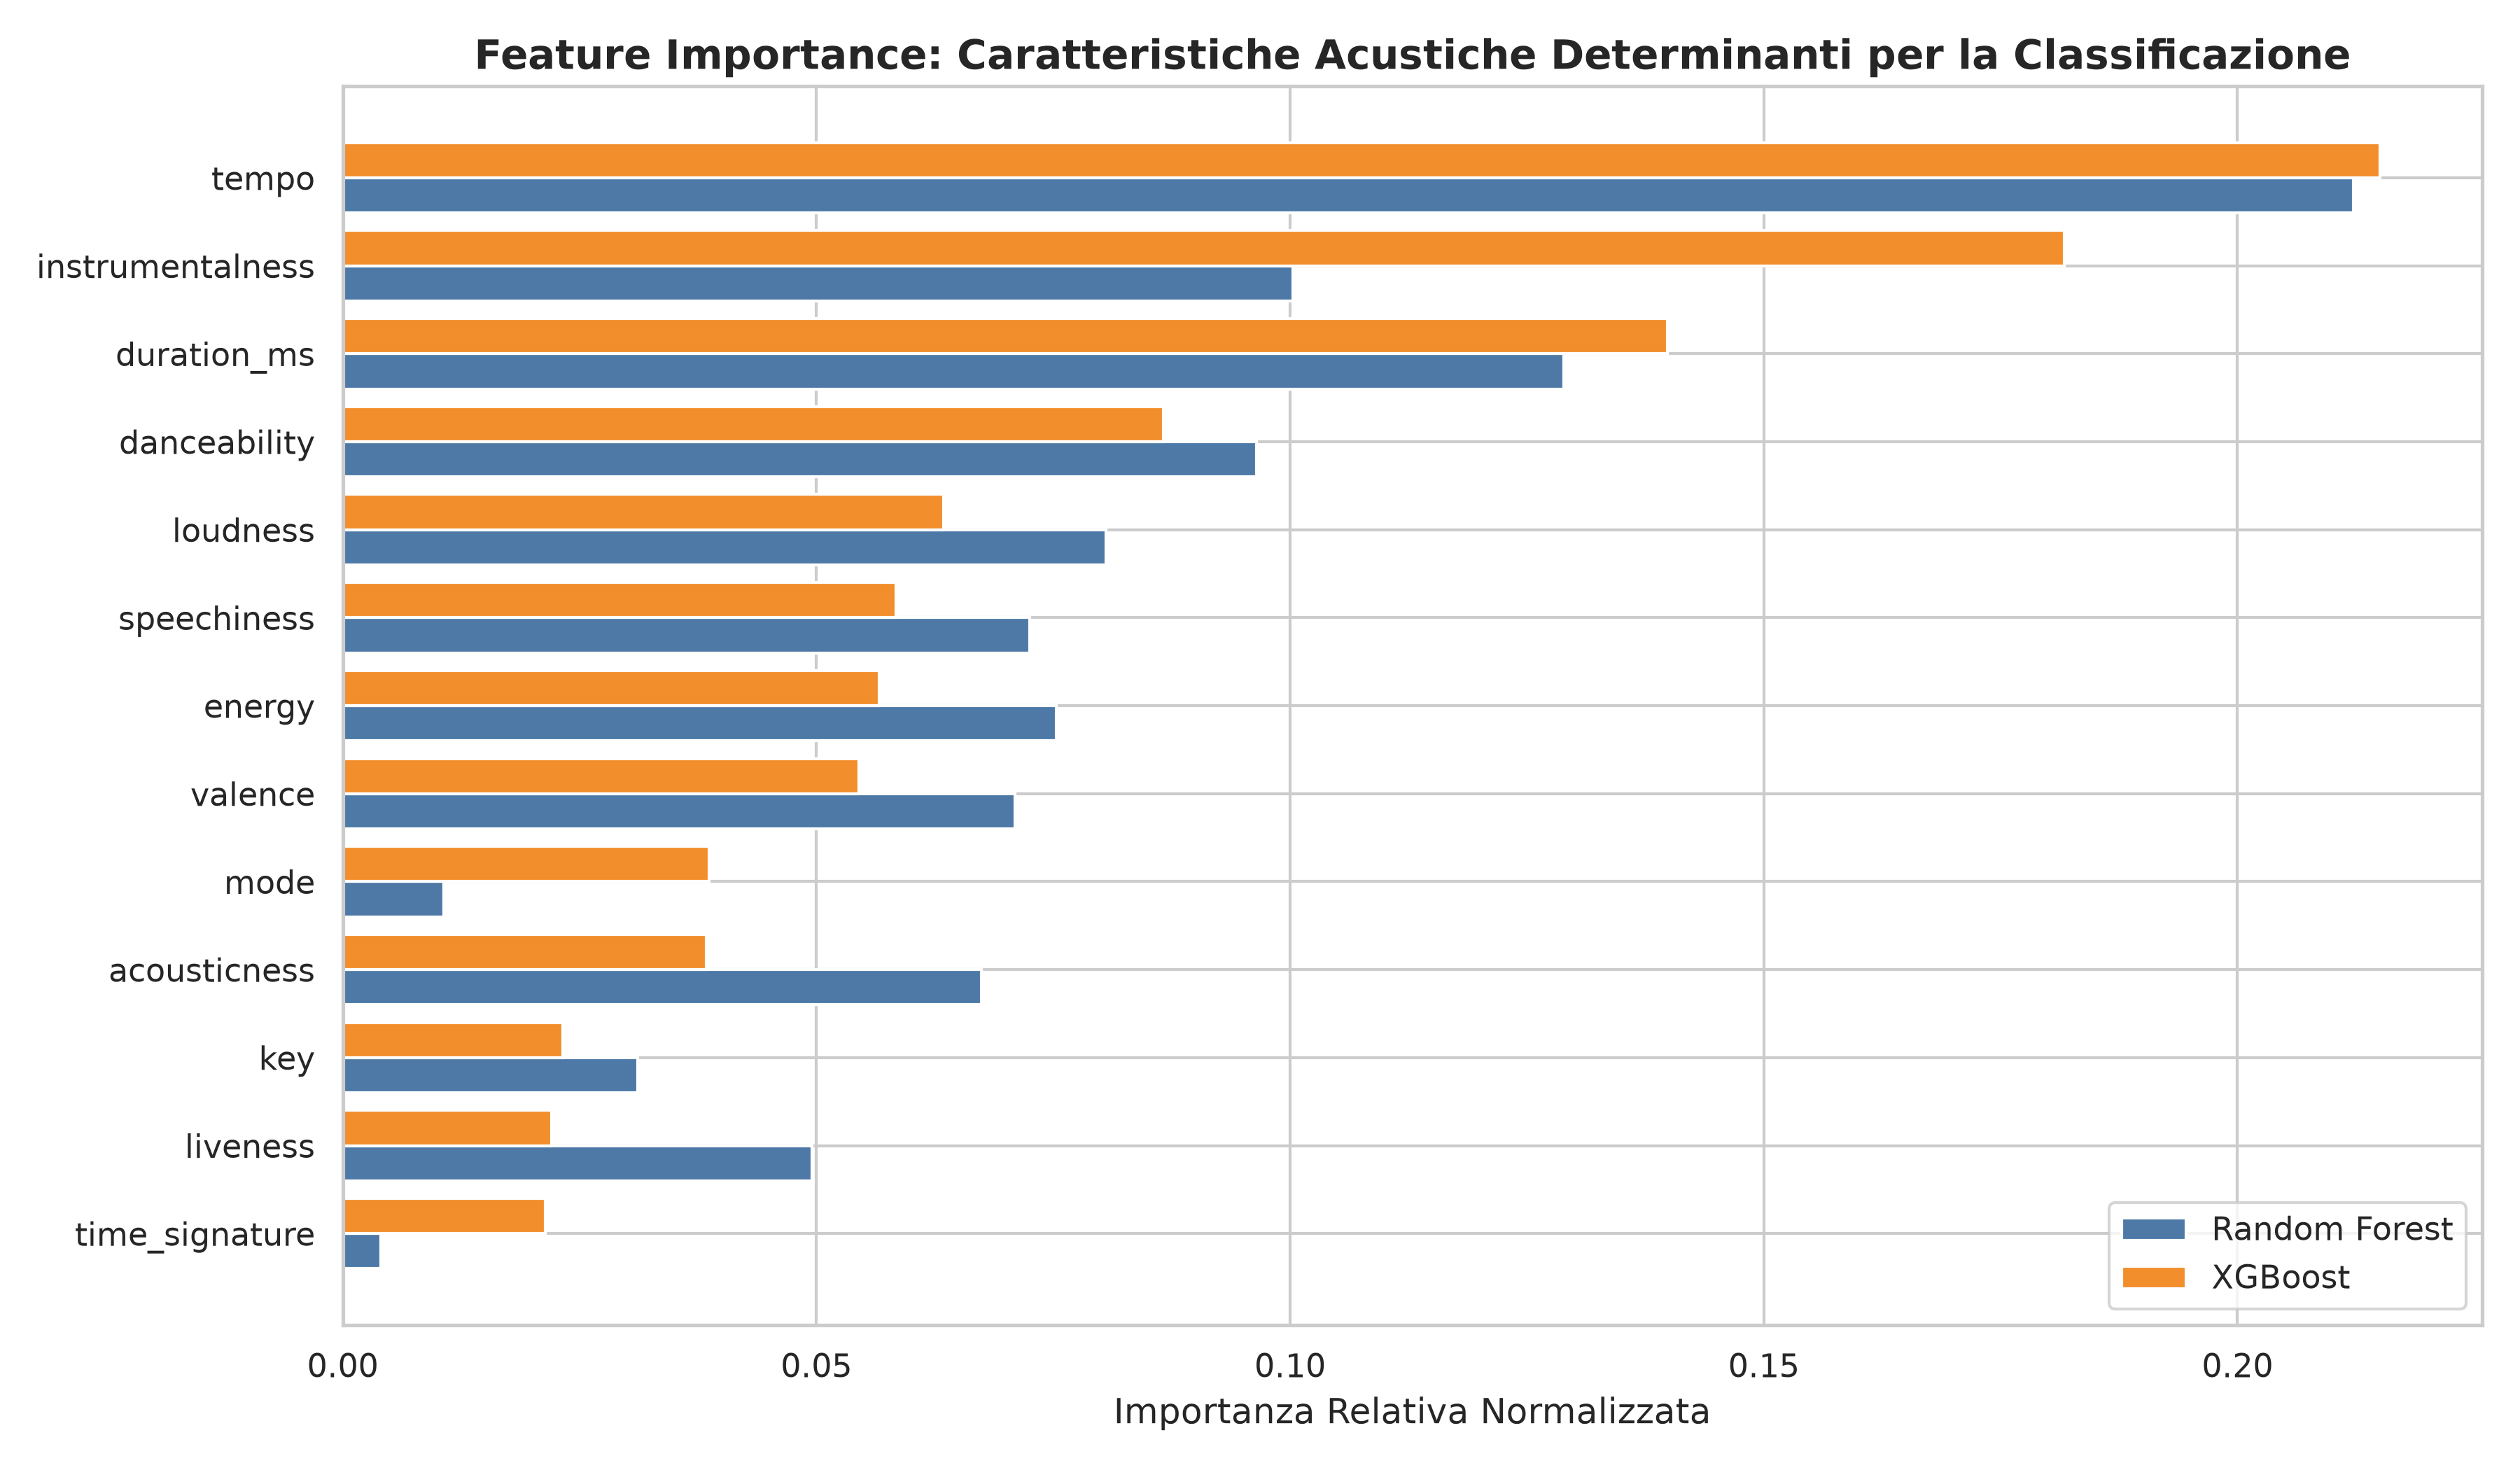
\includegraphics[width=0.85\textwidth]{capitolo3/img/fig13_feature_importance.png}
    \caption{Feature Importance: confronto dei contributi percentuali tra Random Forest e XGBoost.}
    \label{fig:feature_importance}
\end{figure}

Dalla Figura \ref{fig:feature_importance} si evince chiaramente quali siano i fattori più discriminanti:
\begin{itemize}
    \item \texttt{tempo} (BPM): Risulta in assoluto la feature con il peso informativo più alto per entrambi i modelli. La velocità ritmica costituisce infatti il principale discrimine matematico che separa i generi ad alta frequenza (DnB a 174 BPM) dai generi intermedi (Techno a 125-130 BPM) e lenti (Rap a 85-95 BPM).
    \item \texttt{speechiness}: Isola in modo netto il mondo Hip-Hop, Rap e Trap (ad alto contenuto verbale) dai generi dance interamente strumentali.
    \item \texttt{danceability}, \texttt{loudness} ed \texttt{energy}: Determinano la compattezza ritmica, la pressione acustica e l'impatto sonoro percepito.
    \item Al contrario, \texttt{key}, \texttt{mode} e \texttt{time\_signature} presentano un'importanza marginale, a riprova del fatto che la tonalità o la modalità maggiore/minore non vincolano in modo univoco il genere musicale di appartenenza.
\end{itemize}

\newpage
% =========================================================================
% SEZIONE 3.4: EVOLUZIONE DEL MODELLO - CLASSIFICAZIONE GERARCHICA
% =========================================================================
\subsection{Evoluzione del Modello: Classificazione Gerarchica e Modelli Specialisti}

\noindent\textit{Nota metodologica sui riferimenti visivi: Si precisa preliminarmente che tutti i grafici e gli elaborati diagnostici presentati e discussi all'interno della presente sezione sono consultabili e archiviati nella cartella \texttt{figures\_contu} del repository di progetto.}

\vspace{0.3cm}
L'analisi critica condotta nelle sezioni precedenti ha posto in luce un'evidenza empirica di fondamentale rilievo: sebbene l'architettura di Ensemble Learning (Voting e Stacking Classifier) abbia permesso di raggiungere un'accuratezza ragguardevole del \textbf{68.90\%} sui 15 generi musicali di partenza (a fronte di una baseline probabilistica casuale del $6.67\%$), l'esame approfondito della matrice di confusione (Figura \ref{fig:confusion_matrix}) rivela che gli errori di classificazione non sono distribuiti in maniera casuale né uniforme nello spazio ipersferico delle classi. Al contrario, la quasi totalità dei falsi positivi e dei falsi negativi si manifesta sistematicamente all'interno di cluster di sottogeneri caratterizzati da un'evidente parentela stilistica e produttiva, quali le costanti intersezioni tra \textit{Rap}, \textit{Underground Rap}, \textit{Dark Trap} e \textit{Trap Metal}, oppure le sovrapposizioni tra i sottogeneri del clubbing elettronico.

Tale riscontro dimostra che l'approccio ``piatto'' (\textit{flat multiclass classification}) soffre di un limite concettuale: costringere un singolo modello a tracciare contemporaneamente superfici decisionali che separino macro-universi sonori radicalmente eterogenei (ad esempio un brano Drum and Bass da una traccia Pop) e, al contempo, micro-differenze sottili tra sottogeneri stilisticamente contigui genera una complessa interferenza di confine (\textit{boundary confusion}). 

Per superare tale problematica e disarticolare la complessità dello spazio decisionale, è stata introdotta un'architettura di \textbf{classificazione gerarchica a due stadi} (\textit{two-stage hierarchical cascade}):
\begin{enumerate}
    \item \textbf{Livello 1 (Macro-Generi):} Un classificatore supervisionato d'insieme deputato all'identificazione della macro-famiglia acustica di appartenenza;
    \item \textbf{Livello 2 (Modelli Specialisti Intra-Famiglia):} Un pool di modelli specialistici indipendenti, ciascuno istanziato ed ottimizzato esclusivamente all'interno del perimetro della singola macro-famiglia, preposto alla discriminazione fine dei relativi sottogeneri.
\end{enumerate}

\subsubsection{Livello 1: Classificazione delle Macro-Famiglie}

Al fine di aggregare categorie acusticamente affini, i 15 generi originali sono stati ricondotti a 4 ampie e coerenti Macro-Famiglie musicali:
\begin{itemize}
    \item \textbf{Urban/Rap:} comprendente \textit{Dark Trap}, \textit{Hiphop}, \textit{Rap}, \textit{RnB}, \textit{Trap Metal}, \textit{Underground Rap} e \textit{trap};
    \item \textbf{Electronic/Club:} comprendente \textit{psytrance}, \textit{techhouse}, \textit{techno} e \textit{trance};
    \item \textbf{Bass/Hard:} comprendente le produzioni ad alta pressione ritmica \textit{dnb} e \textit{hardstyle};
    \item \textbf{Pop/Alternative:} comprendente i filoni vocali e melodici \textit{Emo} e \textit{Pop}.
\end{itemize}

Su tale configurazione a 4 classi è stato riaddestrato il modello d'insieme (Voting Classifier a Soft Voting). I risultati ottenuti certificano un salto prestazionale straordinario: l'accuratezza globale sul Test Set passa dal precedente 68.90\% a un ragguardevole \textbf{89.4\%}.

\begin{figure}[H]
    \centering
    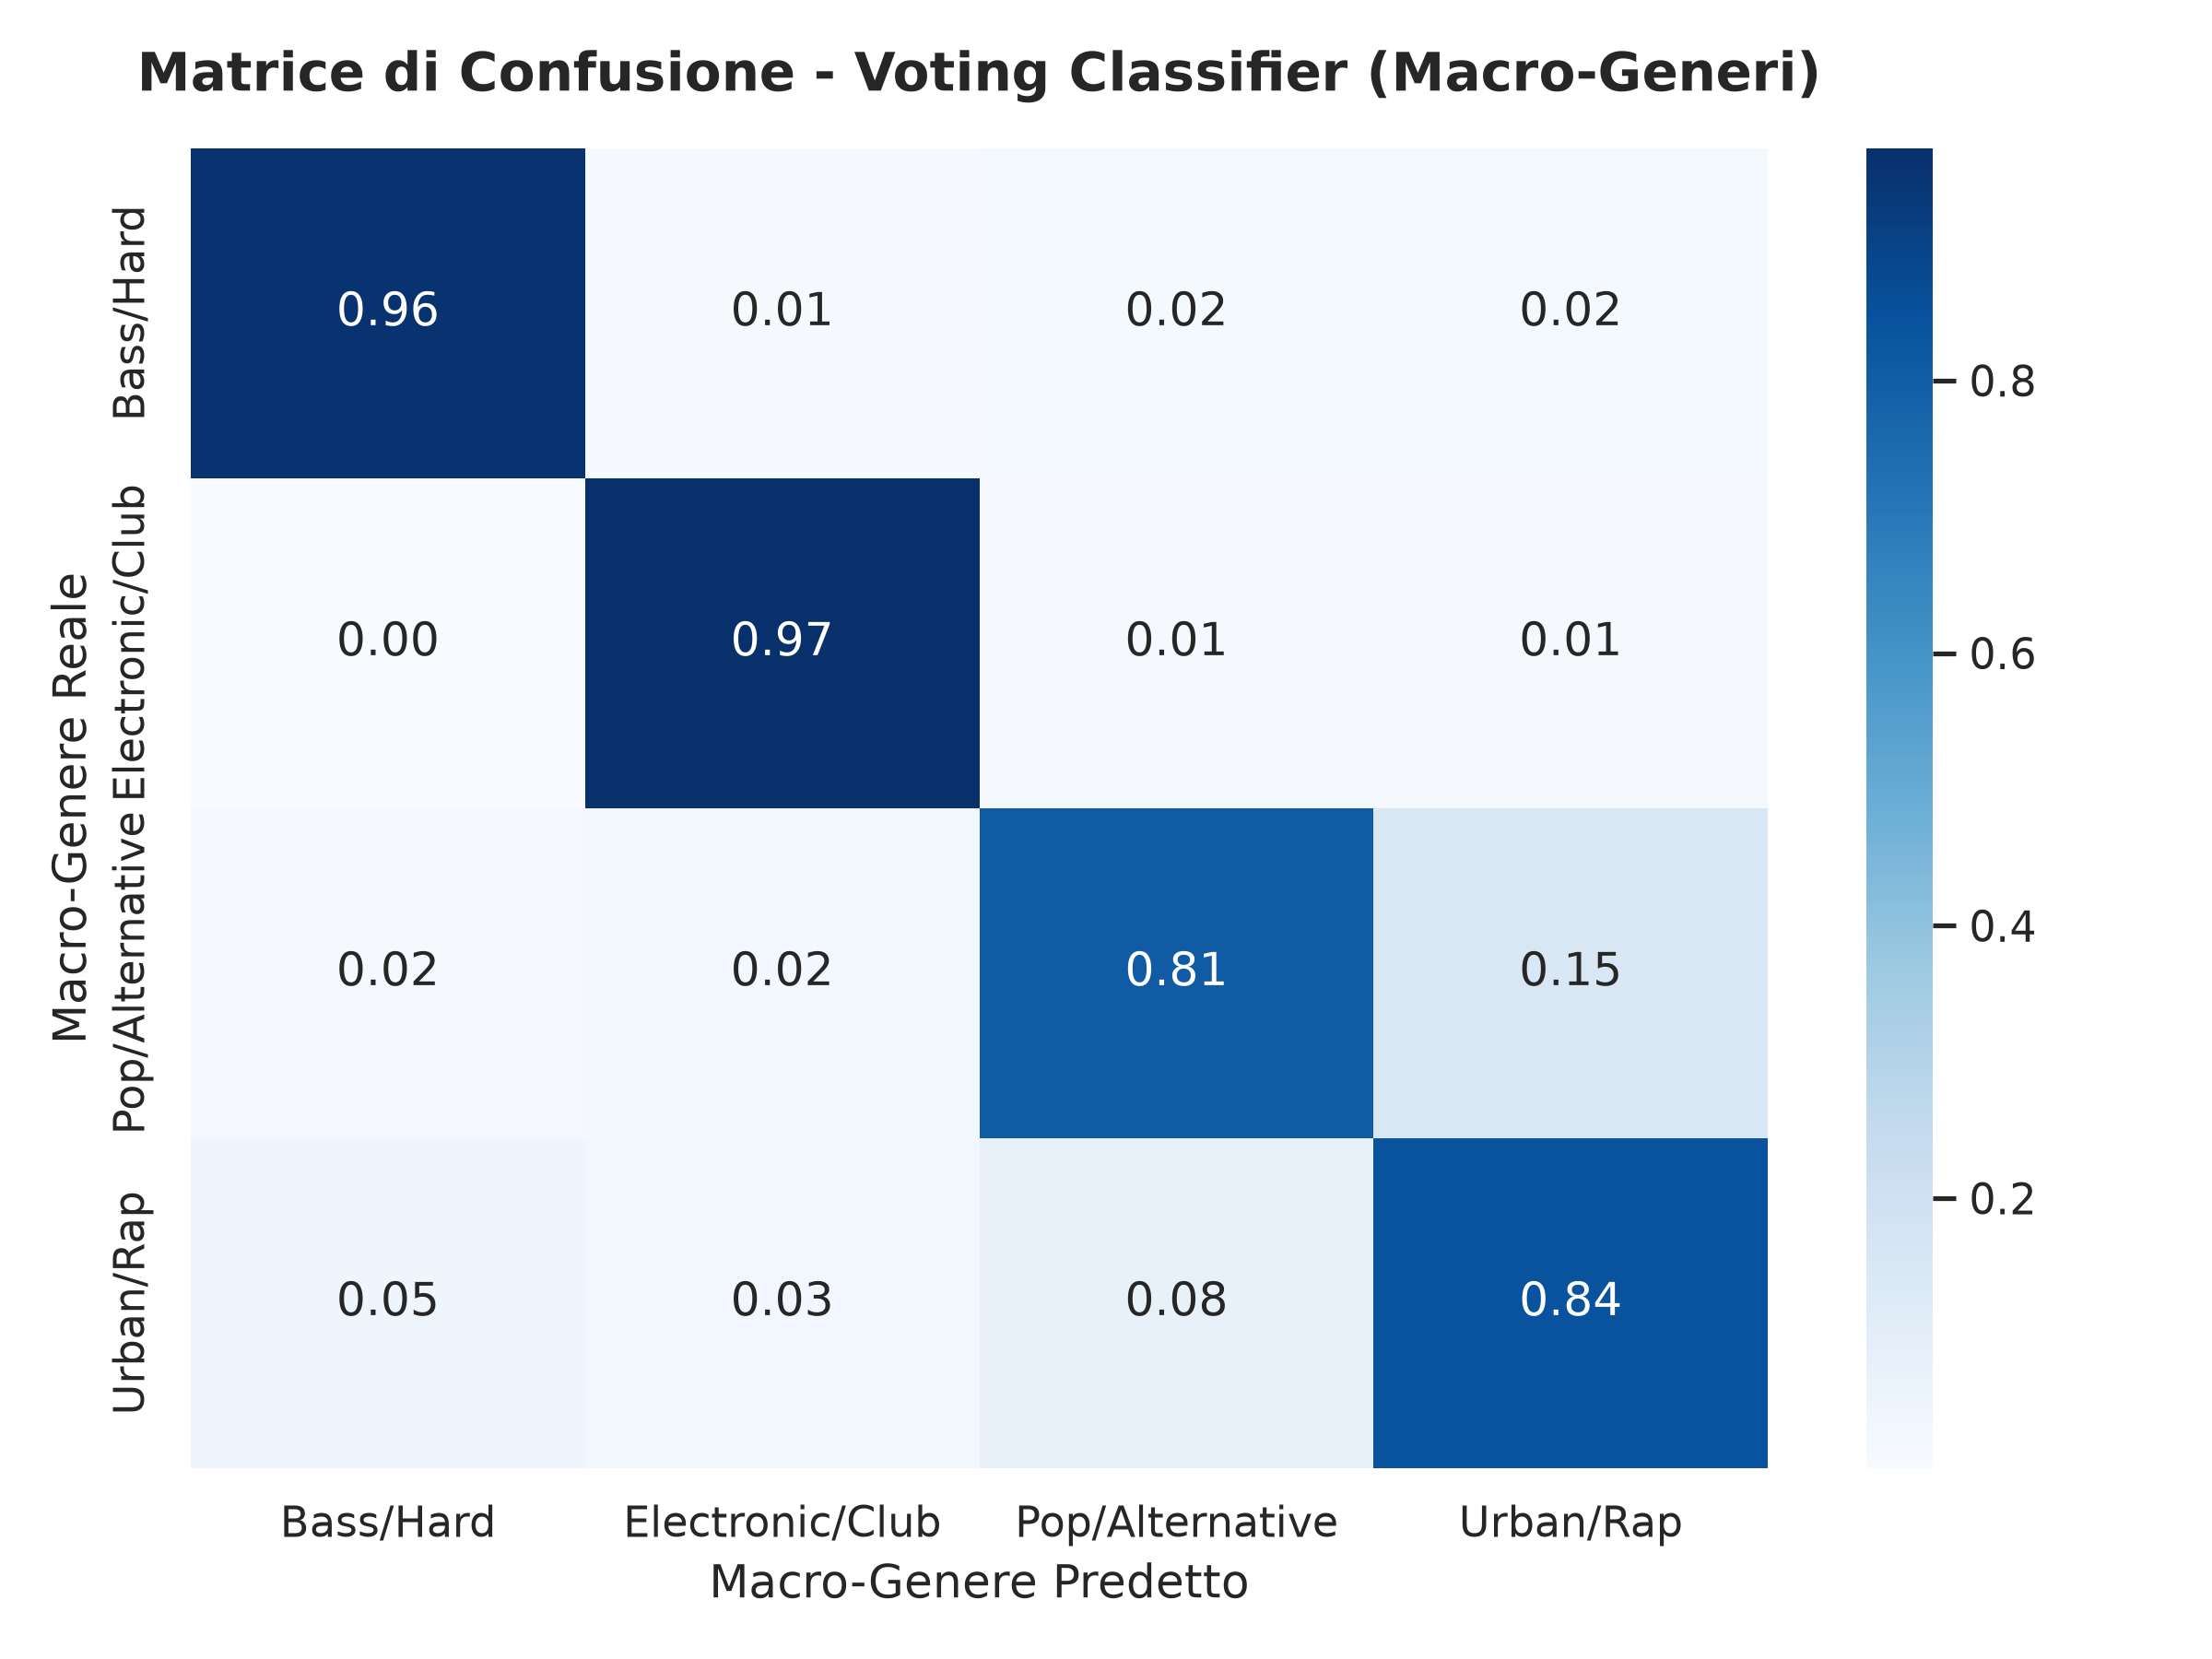
\includegraphics[width=0.78\textwidth]{figures_contu/fig08_confusion_matrix_macro.png}
    \caption{Matrice di confusione normalizzata del Voting Classifier sulle 4 Macro-Famiglie (archivio \texttt{figures\_contu/fig08\_confusion\_matrix\_macro.png}).}
    \label{fig:confusion_matrix_macro}
\end{figure}

L'analisi della Figura \ref{fig:confusion_matrix_macro} evidenzia una concentrazione di probabilità quasi perfetta lungo la diagonale principale:
\begin{itemize}
    \item La famiglia \textbf{Electronic/Club} raggiunge un'accuratezza del \textbf{97\%}, manifestando una separazione praticamente totale rispetto a tutti gli altri stili;
    \item La famiglia \textbf{Bass/Hard} registra una precisione del \textbf{96\%}, a testimonianza di come i profili estremi di tempo e densità acustica isolino il cluster da qualunque interferenza;
    \item La famiglia \textbf{Urban/Rap} si attesta all'\textbf{84\%} di recall corretta, con una dispersione trascurabile confinata verso Pop/Alternative ($8\%$) e Bass/Hard ($5\%$);
    \item La famiglia \textbf{Pop/Alternative} si attesta all'\textbf{81\%}, evidenziando una fisiologica confluenza del $15\%$ verso l'Urban/Rap, motivata dalla presenza di canzoni Pop contemporanee con cadenze vocali e basi ritmiche marcatamente mutuate dall'RnB e dalla musica urbana.
\end{itemize}

\begin{figure}[H]
    \centering
    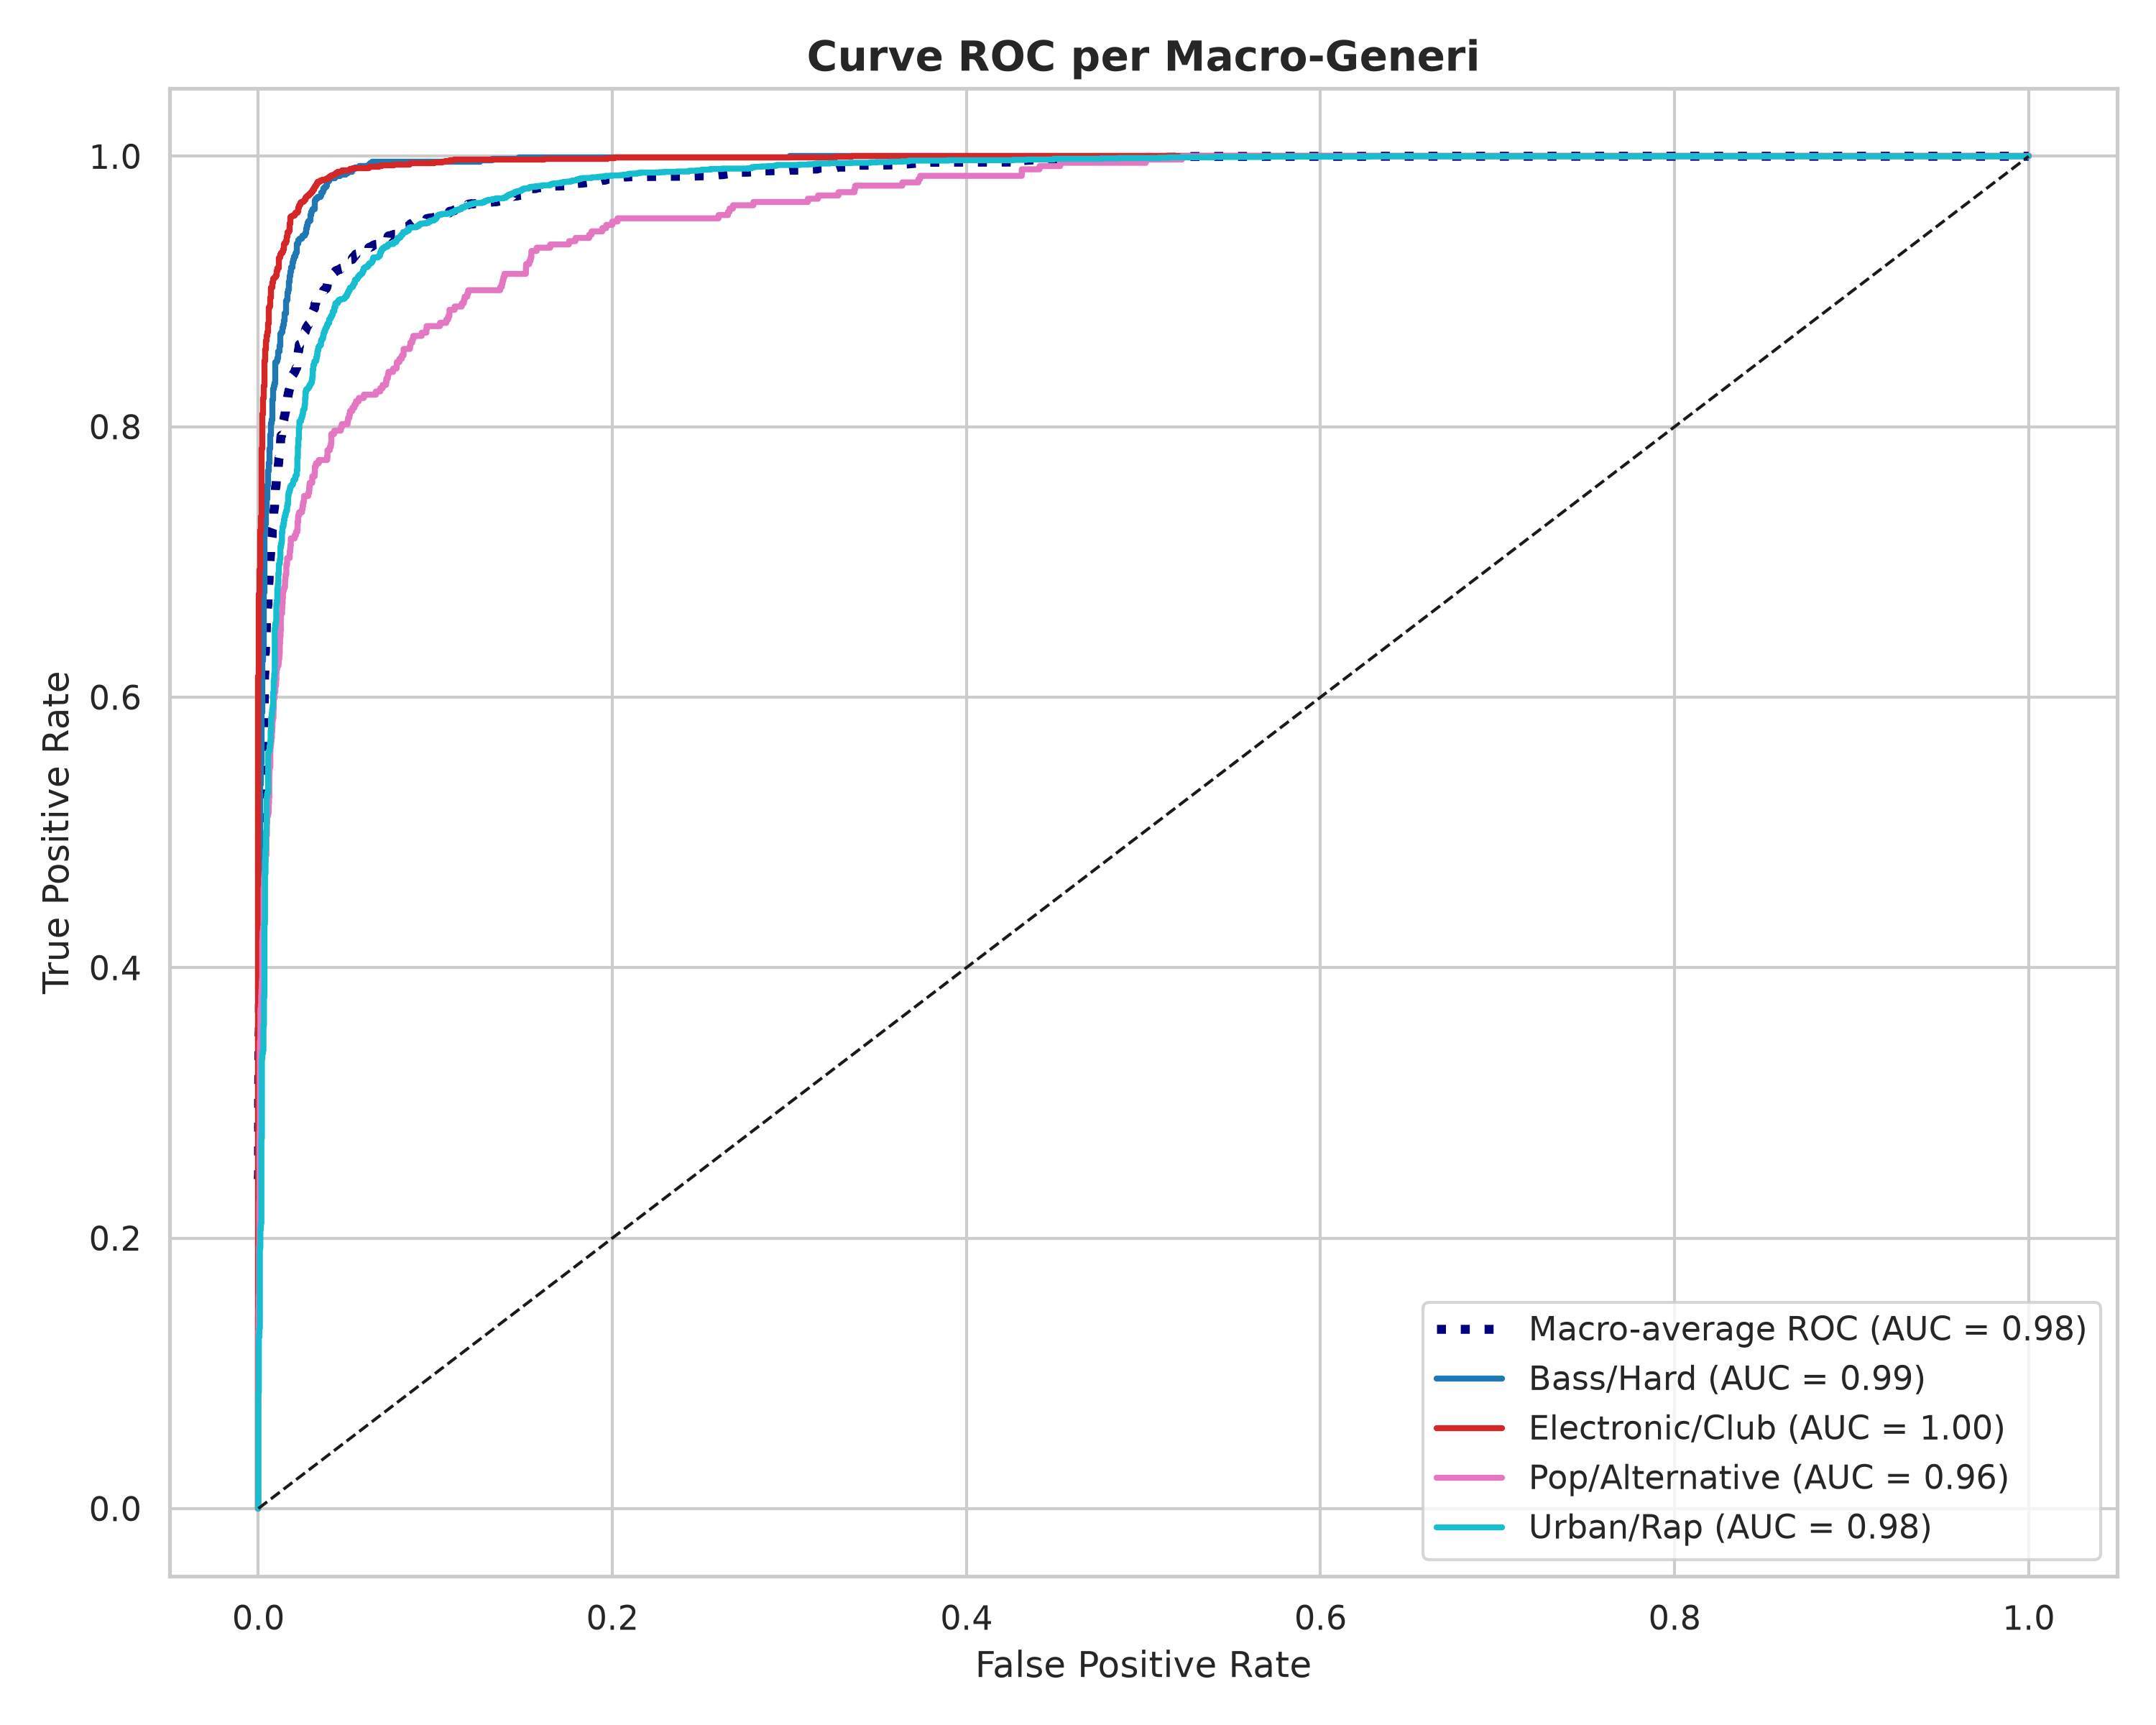
\includegraphics[width=0.78\textwidth]{figures_contu/fig10_roc_curves_macro.png}
    \caption{Curve ROC One-vs-Rest per le 4 Macro-Famiglie, con un AUC medio globale pari a 0.98 (archivio \texttt{figures\_contu/fig10\_roc_curves_macro.png}).}
    \label{fig:roc_macro}
\end{figure}

L'eccellenza discriminante al Livello 1 è pienamente corroborata dall'analisi delle curve ROC riportate in Figura \ref{fig:roc_macro}: il valore di \textbf{Macro-Average ROC-AUC raggiunge l'eccezionale quota di 0.98}. Nello specifico, la curva della famiglia \textit{Electronic/Club} converge a un AUC perfetto di \textbf{1.00}, seguita da \textit{Bass/Hard} con \textbf{0.99}, \textit{Urban/Rap} con \textbf{0.98} e \textit{Pop/Alternative} con \textbf{0.96}.

\begin{figure}[H]
    \centering
    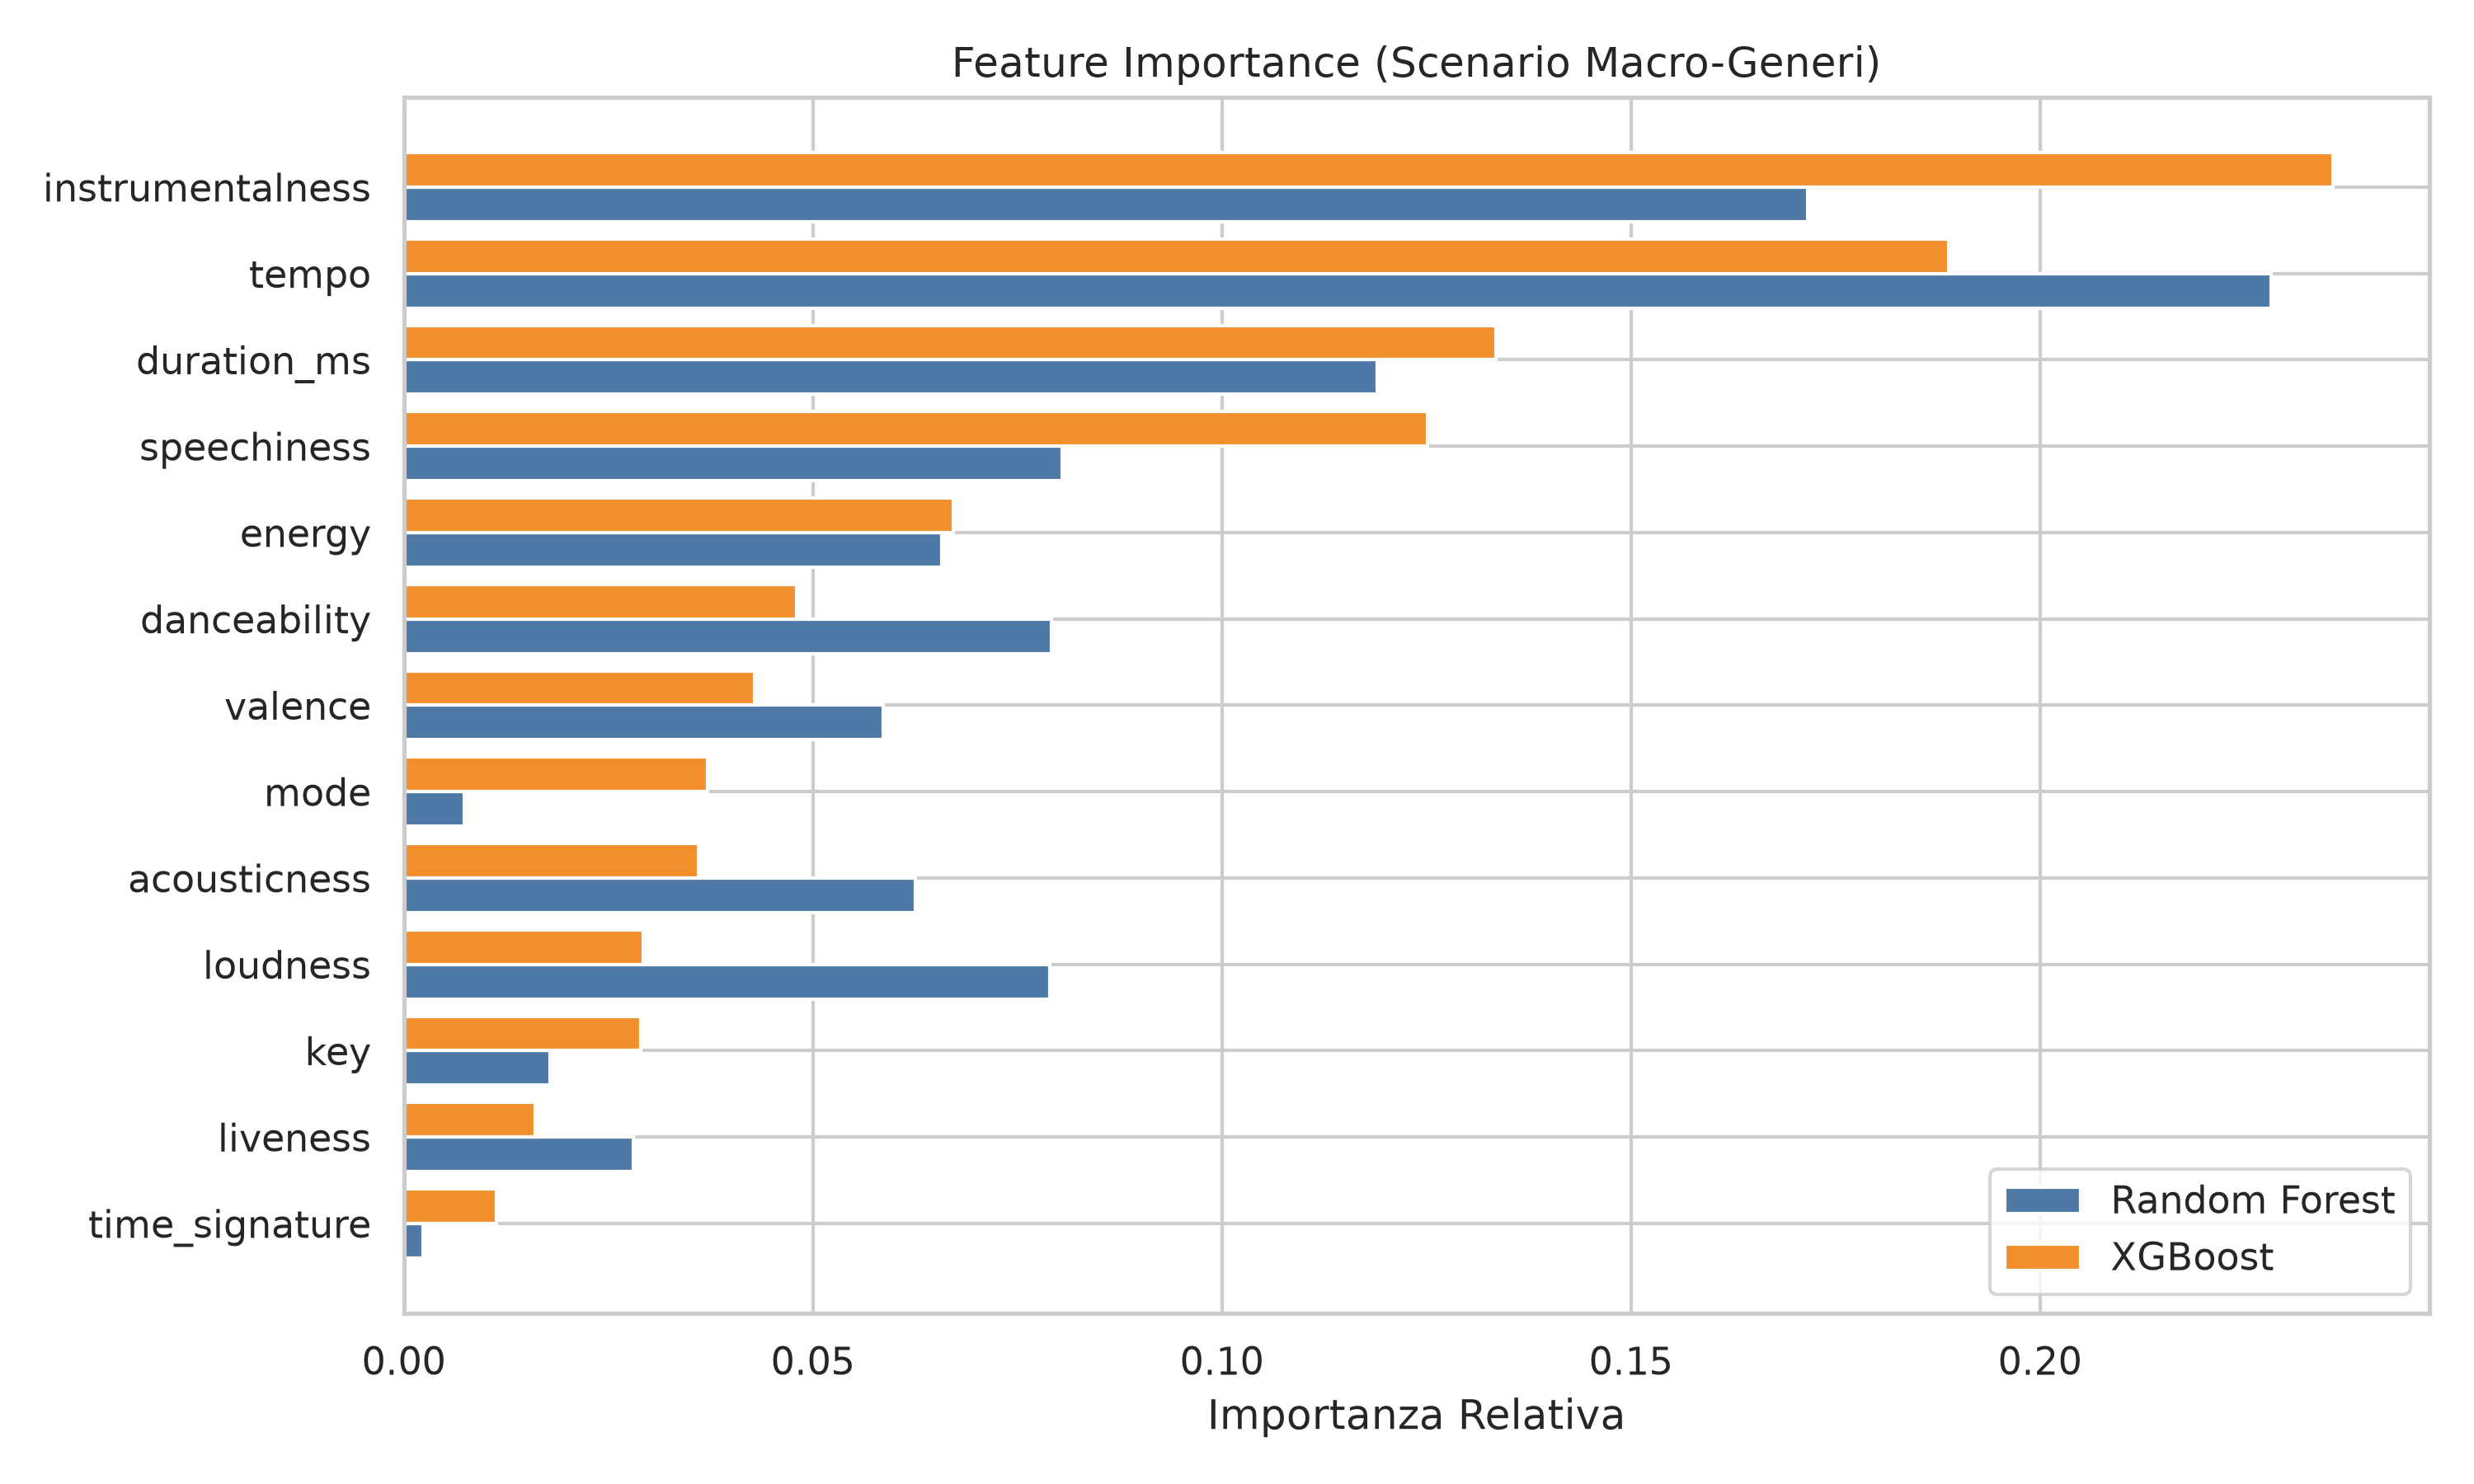
\includegraphics[width=0.85\textwidth]{figures_contu/fig13_feature_importance_macro.png}
    \caption{Importanza relativa delle feature per lo scenario a Macro-Generi calcolata da Random Forest e XGBoost (archivio \texttt{figures\_contu/fig13\_feature_importance_macro.png}).}
    \label{fig:feature_importance_macro}
\end{figure}

La ragione fisica e matematica di tale drastico incremento di performance è esplicitata dal grafico di Feature Importance di Figura \ref{fig:feature_importance_macro}. Mentre nello scenario atomico a 15 generi il modello era costretto a ricorrere quasi unicamente al fattore ritmico, a livello macro la partizione dello spazio decisionale si basa su divergenze acustiche polarizzanti e nette:
\begin{enumerate}
    \item \texttt{instrumentalness}: rappresenta in assoluto la feature cardine (contribuendo per circa il $24\%$ nel modello XGBoost e il $17\%$ in Random Forest), consentendo di discriminare istantaneamente il mondo clubbing e strumentale dalle categorie vocal-oriented;
    \item \texttt{tempo}: si conferma primario (oltre il $22\%$ per Random Forest e il $19\%$ per XGBoost), separando con nettezza le dinamiche iper-cinetiche del Bass/Hard dalle velocità cadenzate delle altre produzioni;
    \item \texttt{speechiness}: con un contributo vicino al $13\%$ in XGBoost, definisce la linea di faglia strutturale tra la metrica parlata e ritmicamente densa dell'Urban/Rap e i testi melodici o rarefatti delle altre famiglie;
    \item \texttt{duration\_ms}: concorre in modo rilevante all'isolamento delle strutture a traccia estesa tipiche dei brani da discoteca rispetto ai formati concisi dell'ascolto radiofonico e streaming.
\end{enumerate}

\newpage
\subsubsection{Livello 2: Modelli Specialisti Intra-Famiglia}

Verificata l'accuratezza dell'89.4\% nell'instradamento al macro-genere corretto, il secondo stadio della pipeline prevede l'attivazione di \textbf{4 modelli XGBoost specialisti}, ciascuno addestrato ed ottimizzato in modo dedicato all'interno dei soli campioni appartenenti a una singola macro-famiglia. L'obiettivo primario di tali modelli consiste nel verificare se, isolando il rumore generato dalle altre famiglie musicali, l'algoritmo sia in grado di cogliere pattern sottili utili a discriminare i sottogeneri interni.

Le matrici di confusione normalizzate prodotte dai quattro specialisti sul Test Set sono illustrate congiuntamente in Figura \ref{fig:specialist_confusion_matrices}.

\begin{figure}[H]
    \centering
    \begin{subfigure}[b]{0.48\textwidth}
        \centering
        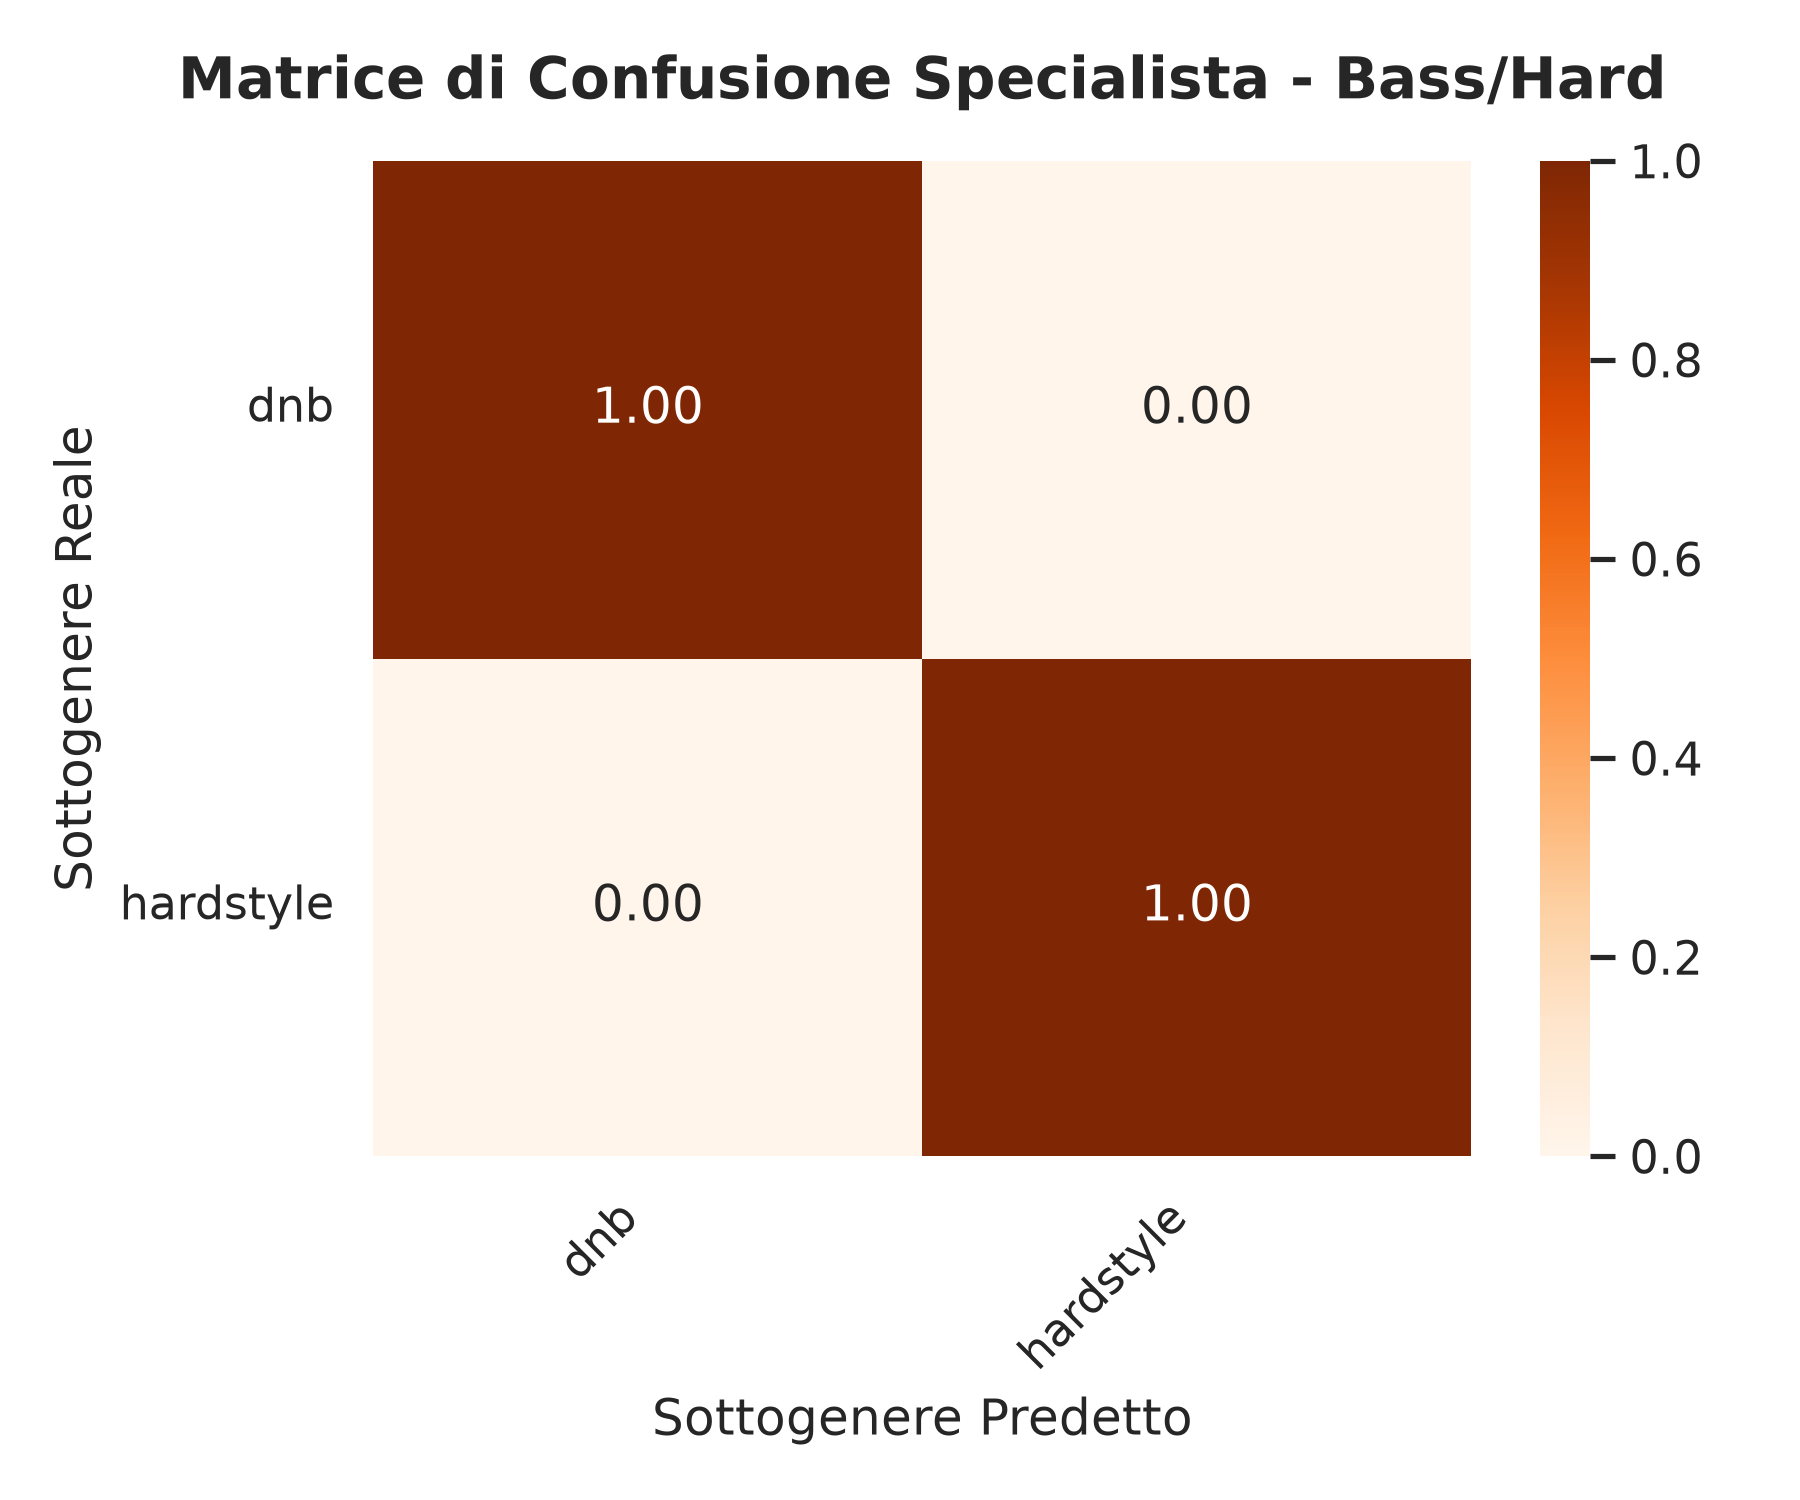
\includegraphics[width=\textwidth]{figures_contu/fig_specialist_cm_Bass_Hard.png}
        \caption{Specialista Bass/Hard (100\% di accuratezza).}
        \label{fig:sp_bass_hard}
    \end{subfigure}
    \hfill
    \begin{subfigure}[b]{0.48\textwidth}
        \centering
        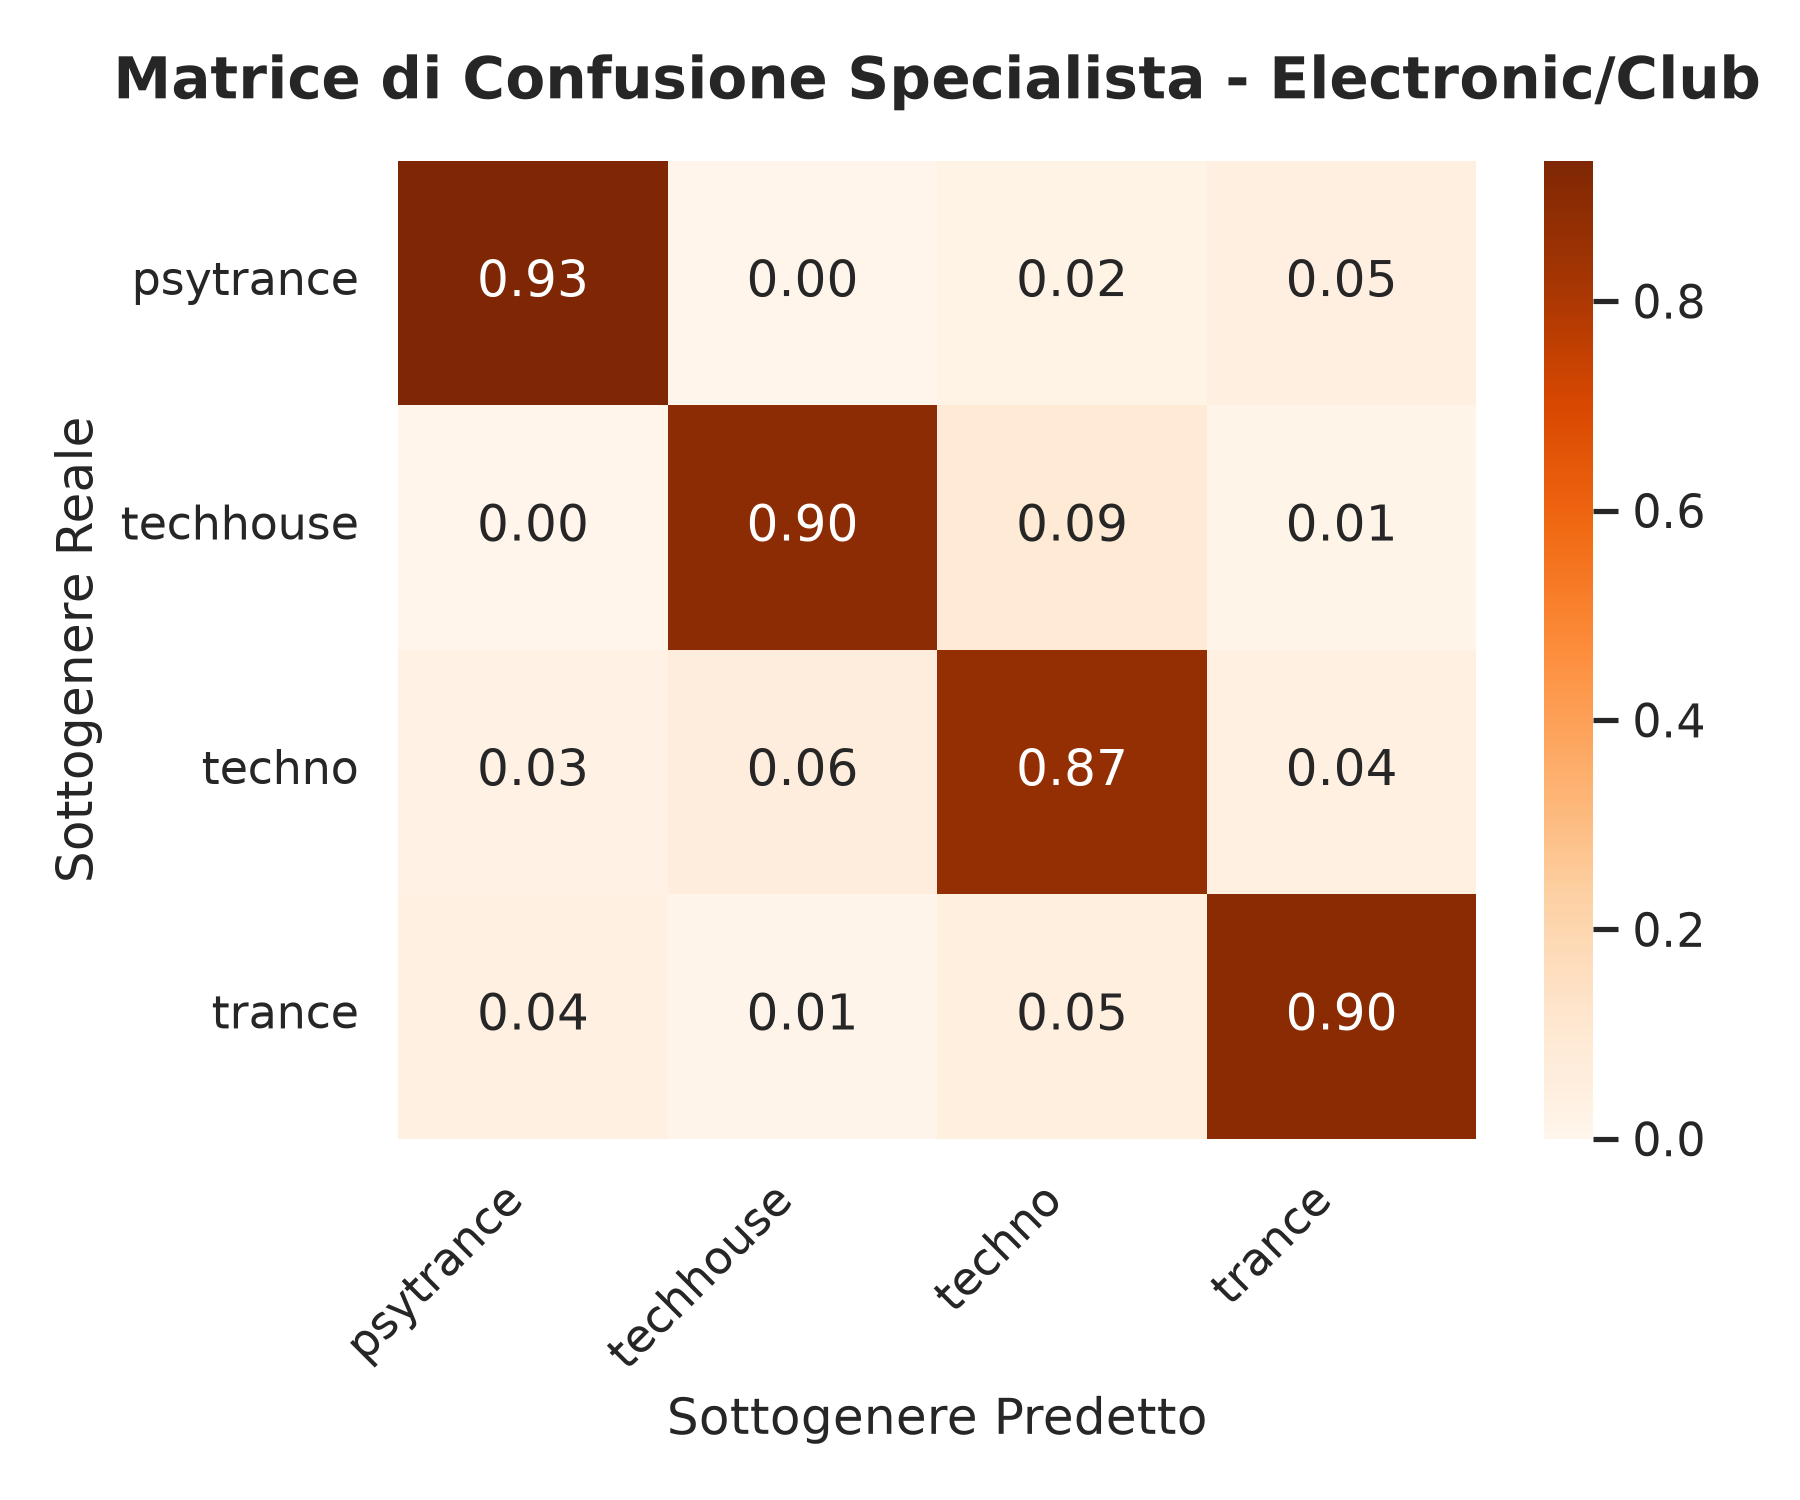
\includegraphics[width=\textwidth]{figures_contu/fig_specialist_cm_Electronic_Club.png}
        \caption{Specialista Electronic/Club (accuratezza $\ge 90\%$).}
        \label{fig:sp_electronic}
    \end{subfigure}
    \\[0.4cm]
    \begin{subfigure}[b]{0.48\textwidth}
        \centering
        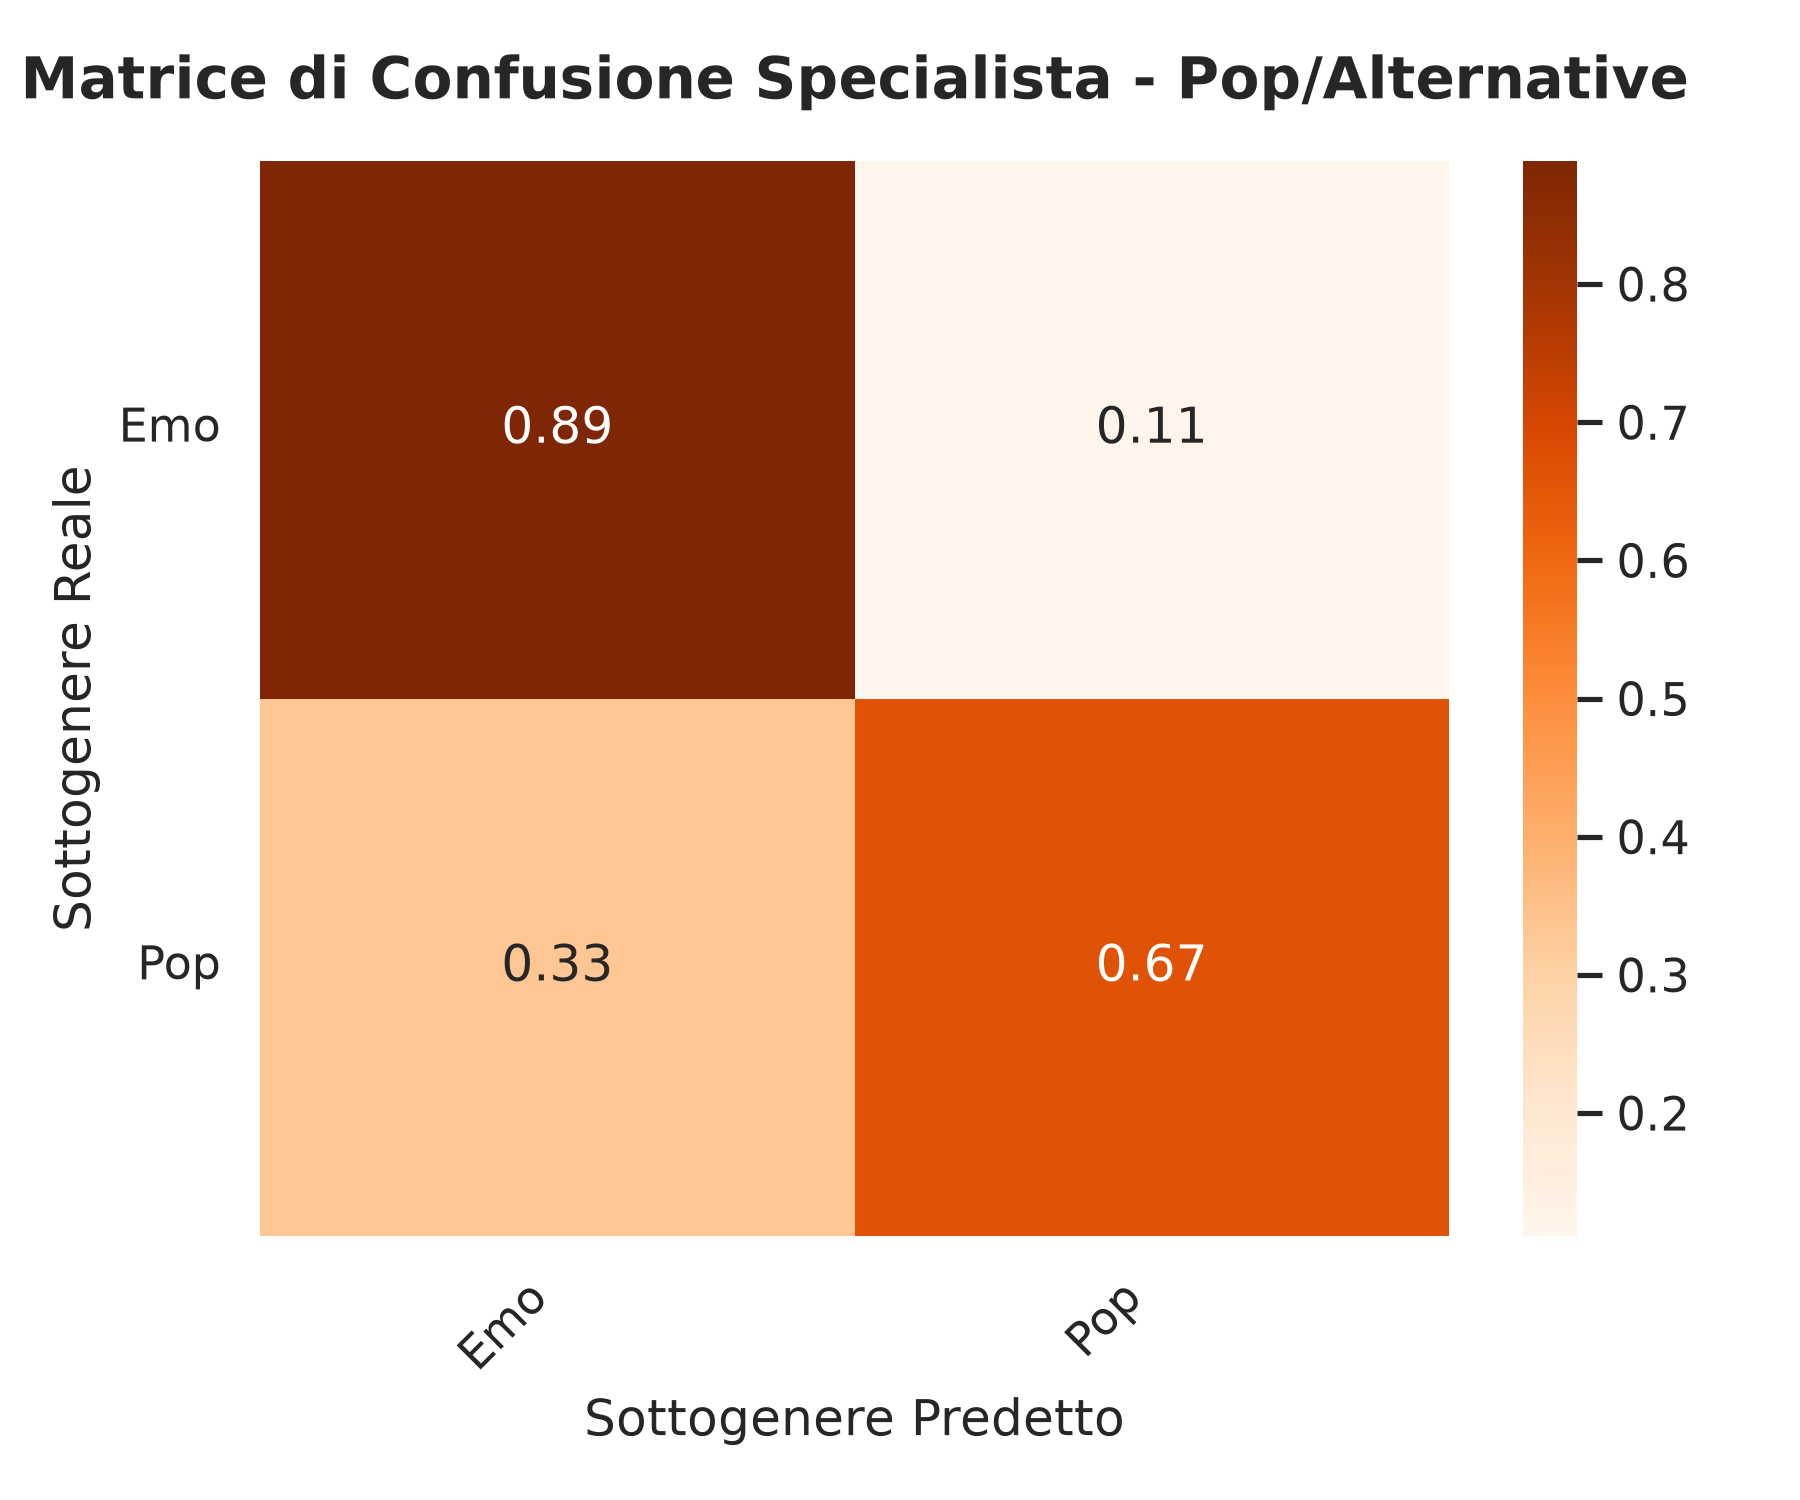
\includegraphics[width=\textwidth]{figures_contu/fig_specialist_cm_Pop_Alternative.png}
        \caption{Specialista Pop/Alternative (Emo vs Pop).}
        \label{fig:sp_pop_alt}
    \end{subfigure}
    \hfill
    \begin{subfigure}[b]{0.48\textwidth}
        \centering
        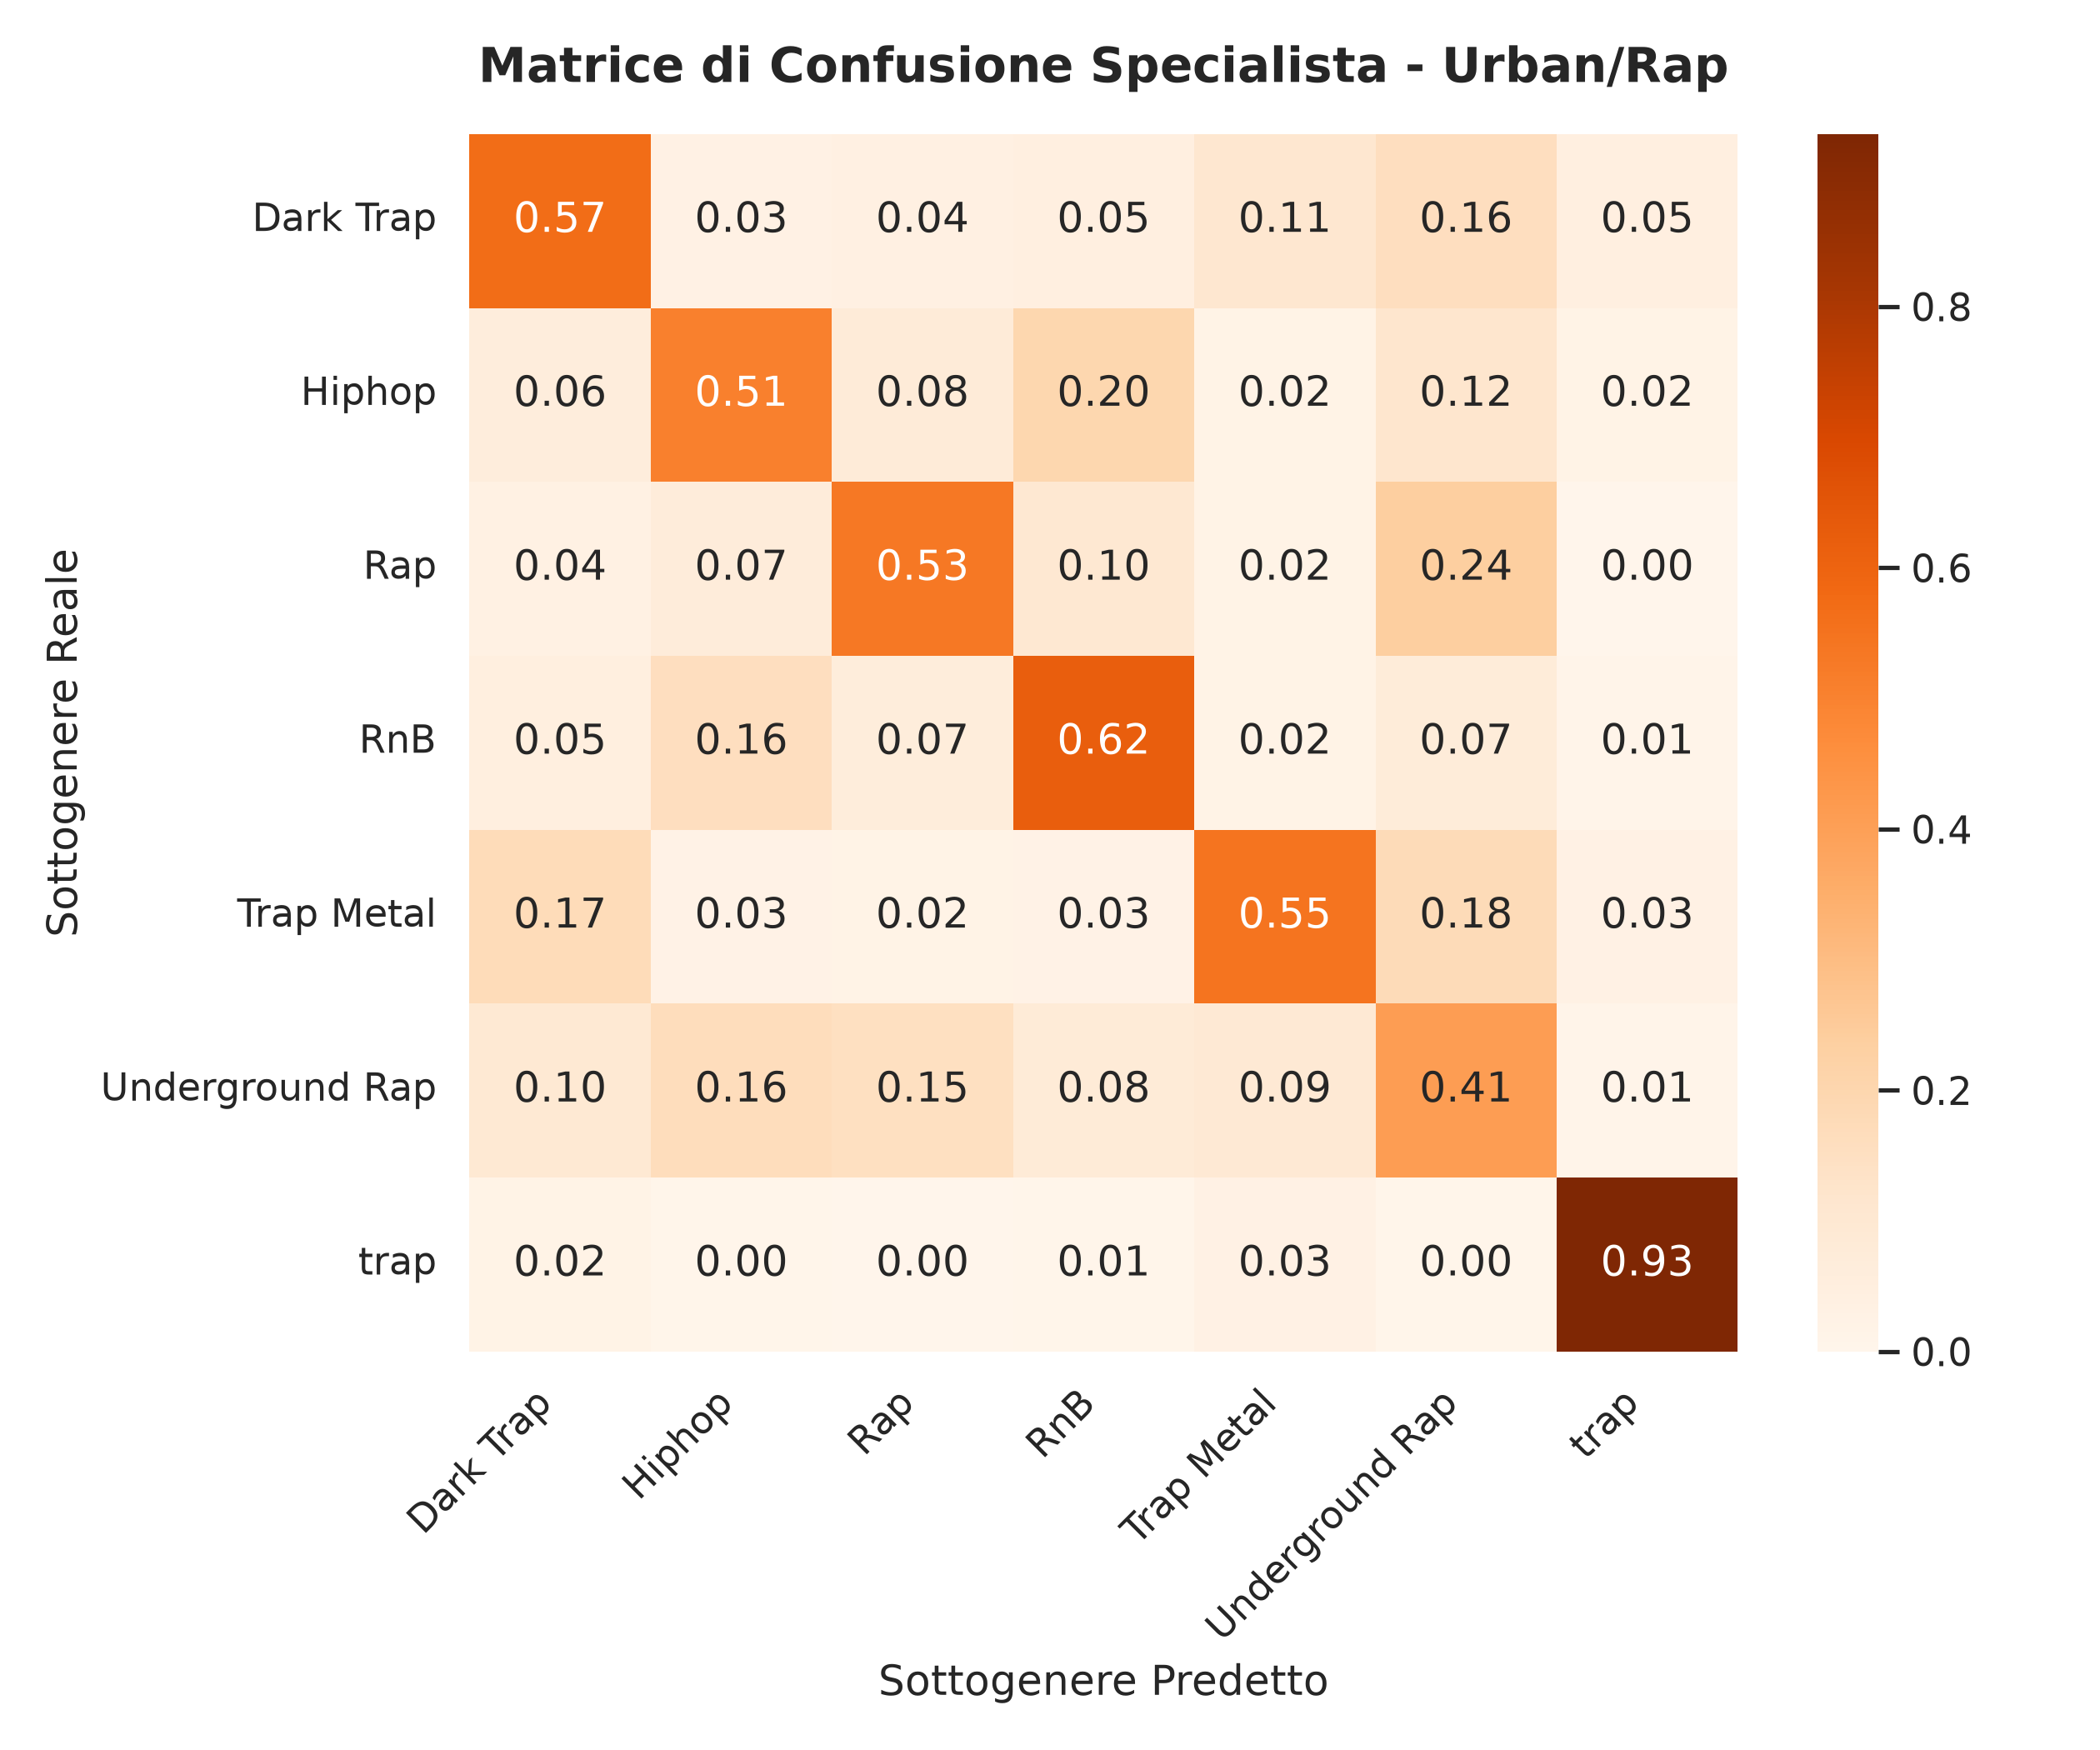
\includegraphics[width=\textwidth]{figures_contu/fig_specialist_cm_Urban_Rap.png}
        \caption{Specialista Urban/Rap (evidente overlap acustico).}
        \label{fig:sp_urban_rap}
    \end{subfigure}
    \caption{Matrici di confusione dei 4 classificatori specialisti XGBoost di Livello 2 addestrati sulle singole macro-famiglie (file della suite \texttt{figures\_contu}).}
    \label{fig:specialist_confusion_matrices}
\end{figure}

Dall'analisi comparativa dei quattro modelli emergono comportamenti profondamente divergenti a seconda della natura intrinseca del genere musicale:
\begin{itemize}
    \item \textbf{Specialista Bass/Hard (Figura \ref{fig:sp_bass_hard}):} Raggiunge un risultato teoricamente e operativamente impeccabile, registrando il \textbf{100\% esatto di accuratezza} su entrambi i sottogeneri (\textit{dnb} = 1.00, \textit{hardstyle} = 1.00) con zero campioni confusi. La netta divergenza tra la ritmica breakbeat a 174 BPM della Drum and Bass e la cassa quadrupla a 150 BPM con saturazione armonica dell'Hardstyle permette allo specialista una separazione perfetta nello spazio delle caratteristiche audio.
    \item \textbf{Specialista Electronic/Club (Figura \ref{fig:sp_electronic}):} Evidenzia una capacità discriminante eccellente, attestandosi costantemente su percentuali attorno o superiori al 90\% di classificazione corretta: \textit{psytrance} al \textbf{93\%}, \textit{techhouse} al \textbf{90\%}, \textit{trance} al \textbf{90\%} e \textit{techno} all'\textbf{87\%}. Le uniche lievi confusioni si manifestano tra \textit{techno} e \textit{techhouse} ($6\%$ e $9\%$), dovute alla comune impostazione 4/4 a battute contigue ($\approx 125-130$ BPM).
    \item \textbf{Specialista Pop/Alternative (Figura \ref{fig:sp_pop_alt}):} Mostra una separazione asimmetrica: mentre la classe \textit{Emo} viene isolata con una solida accuratezza dell'\textbf{89\%}, ben il \textbf{33\% delle tracce etichettate come Pop viene erroneamente attribuito all'Emo} (con il Pop corretto ad appena il 67\%). Tale fenomeno riflette la marcata convergenza stilistica del pop moderno con chitarre acustiche e distorte ed atmosfere malinconiche tipiche del filone emo/alternative.
    \item \textbf{Specialista Urban/Rap (Figura \ref{fig:sp_urban_rap}):} In netto contrasto con i successi degli altri specialisti, all'interno del comparto urbano l'accuratezza subisce un vero e proprio tracollo:
    \begin{itemize}
        \item \textit{Underground Rap} viene riconosciuto correttamente soltanto nel \textbf{41\%} dei casi, disperdendosi in maniera generalizzata verso Rap ($15\%$), Hiphop ($16\%$), Dark Trap ($10\%$) e Trap Metal ($9\%$);
        \item \textit{Rap} registra un'accuratezza di appena il \textbf{53\%}, con il $24\%$ delle proprie osservazioni scambiate per Underground Rap e il $10\%$ per RnB;
        \item \textit{Hiphop} viene predetto con successo solo nel \textbf{51\%} dei casi, mostrando una dispersione critica verso RnB ($20\%$) e Underground Rap ($12\%$);
        \item \textit{Trap Metal} ($55\%$) e \textit{Dark Trap} ($57\%$) evidenziano confusioni incrociate biunivoche con il resto del bacino rap;
        \item L'unica eccezione rilevante è costituita dalla classe \textit{trap} (con un'accuratezza del \textbf{93\%}), la cui tipica ritmica cadenzata con sub-bassi 808 scivolati e triplette di hi-hat a frequenza caratteristica ne preserva la riconoscibilità rispetto al rap classico.
    \end{itemize}
\end{itemize}

\subsubsection{Conclusione Diagnostica e Considerazioni sulla Natura delle Etichette}

La sperimentazione gerarchica condotta conduce a una conclusione diagnostica di fondamentale valore metodologico ed epistemologico per l'intero lavoro di tesi:
\begin{quote}
\textit{L'approccio a cascata a due stadi dimostra inconfutabilmente che l'apparato algoritmico e le tecniche di Machine Learning impiegate sono estremamente validi ed efficaci.}
\end{quote}

Nel momento in cui nel segnale acustico sono presenti differenze timbriche, spettrali e ritmiche oggettive, i modelli di classificazione raggiungono vette di accuratezza prossime o uguali alla perfezione (l'89.4\% a livello macro, con punte del 97\% nell'Electronic e il 100\% nel Bass/Hard).

Alla luce di questa constatazione, il drastico crollo delle performance riscontrato nello specialista \textit{Urban/Rap} non può e non deve essere interpretato come un limite matematico dei modelli predittivi, né come una carenza nel processo di tuning degli iperparametri o nella formulazione del training set. Al contrario, tale esito costituisce la \textbf{formale dimostrazione empirica che i sottogeneri del macro-universo Urban/Rap condividono la medesima, identica impronta e firma acustica}.

Dal punto di vista dell'elaborazione del segnale e dell'estrazione delle caratteristiche sonore (BPM, danceability, energy, loudness, tempo e valence), una traccia classificata da Spotify come \textit{Rap}, \textit{Hiphop} o \textit{Underground Rap} non possiede alcuna differenziazione fisico-armonica misurabile. Le etichette attribuite dalla piattaforma per questa specifica famiglia non riflettono caratteristiche acustiche oggettive, bensì possiedono una valenza prettamente \textbf{culturale, sociologica, contestuale e di marketing editoriale}:
\begin{itemize}
    \item La qualifica di \textit{Underground} rispetto a \textit{Rap} commerciale è determinata dal canale di distribuzione indipendente, dalla notorietà dell'artista e dal target del pubblico, non dal timbro della base musicale;
    \item La demarcazione tematica tra \textit{Dark Trap}, \textit{Trap Metal} o \textit{Hiphop} convenzionale risiede prevalentemente nel contenuto semantico dei testi, nel messaggio sociopolitico e nella crudezza verbale delle rime.
\end{itemize}

Poiché il dataset impiegato è circoscritto alle sole feature ingegneristiche fornite dalle Web API di Spotify e prescinde totalmente dall'analisi del testo (\textit{Natural Language Processing} sulle liriche), il modello si scontra con una frontiera di Bayes intrinsecamente invalicabile: \textbf{non è possibile separare matematicamente ciò che a livello sonoro risulta perfettamente identico}. Tale constatazione sigilla il capitolo con una chiara linea di demarcazione tra ciò che è estraibile dal puro segnale acustico e ciò che appartiene indissolubilmente alla sfera semantico-culturale della musica moderna.

